\section{Appendix for the Coding section}
\label{sec:code_appendix}
\subsection{Measuring human performance on LeetCode}
\label{sec:leetcode-human}
For each question, LeetCode posts its Acceptance rate in terms of the number of accepted submissions over the total number of all submissions. However, we contend that this statistic may be an \emph{improper} benchmark due to the following reason: Each question's Acceptance rate accounts for all historical submissions, and we observe the Acceptance rates of Hard questions is usually higher than that of Medium questions. We speculate that many of the accepted submission could be ``copied-and-pasted" after the solutions are released.
    \item 
%Additionally, the accuracy of human coders on Hard problems is \emph{much higher}, but this may reflect survivor bias -- Only those who have high coding skills would try to solve these questions.  (Not true anymore)
\begin{table}[h]
\centering
\tiny
\begin{tabular}{ccc|ccc|ccc|ccc|ccc}
\hline
\multicolumn{3}{c|}{Contest} &  \multicolumn{3}{c|}{Problem 1} & \multicolumn{3}{c|}{Problem 2} & \multicolumn{3}{c|}{Problem 3} & \multicolumn{3}{c}{Problem 4}\\
\hline
Date & Name & Users\^* & Level & Accepted & \% & Level & Accepted & \% & Level & Accepted & \% & Level & Accepted & \% \\
\hline
8-Oct & 314 & 14499  & Easy & 10630 & 73 & Medium & 9111 & 63 & Medium & 2124 & 15 & Hard & 2132 & 15 \\
15-Oct & Bi 89 & 11050  & Easy & 8022 & 73 & Medium & 4770 & 43 & Medium & 1459 & 13 & Hard & 192 & 2 \\
15-Oct &  315 & 17284  & Easy & 11930 & 69 & Medium & 11079 & 64 & Medium & 9496 & 55 & Hard & 1370 & 8 \\
22-Oct &  316 & 14823  & Easy & 9503 & 64 & Medium & 6110 & 41 & Hard & 1550 & 10 & Hard & 1437 & 10 \\
29-Oct & Bi 90 & 10763  & Easy & 7822 & 73 & Medium & 6902 & 64 & Medium & 3138 & 29 & Hard & 743 & 7 \\
29-Oct &  317 & 15767  & Easy & 10900 & 69 & Medium & 5959 & 38 & Medium & 4315 & 27 & Hard & 594 & 4 \\
5-Nov &  318 & 15723  & Easy & 11024 & 70 & Medium & 6454 & 41 & Medium & 3668 & 23 & Hard & 345 & 2 \\
12-Nov & Bi 91 & 12527  & Easy & 9820 & 78 & Medium & 3696 & 30 & Medium & 1141 & 9 & Hard & 291 & 2 \\
12-Nov &  319 & 15723  & Easy & 11024 & 70 & Medium & 6454 & 41 & Medium & 3668 & 23 & Hard & 345 & 2 \\
19-Nov &  320 & 13866  & Easy & 9355 & 67 & Medium & 4931 & 36 & Medium & 1571 & 11 & Hard & 488 & 4 \\
26-Nov & Bi 92 & 10769  & Easy & 8276 & 77 & Medium & 6206 & 58 & Medium & 4820 & 45 & Hard & 492 & 5 \\
26-Nov &  321 & 12958  & Easy & 8605 & 66 & Medium & 6986 & 54 & Medium & 5927 & 46 & Hard & 1457 & 11 \\
3-Dec &  322 & 13425  & Easy & 9058 & 67 & Medium & 8238 & 61 & Medium & 3952 & 29 & Hard & 403 & 3 \\
10-Dec & Bi 93 & 10918  & Easy & 8643 & 79 & Medium & 3720 & 34 & Medium & 3210 & 29 & Hard & 170 & 2 \\
10-Dec & 323 & 11415  & Easy & 7791 & 68 & Medium & 5731 & 50 & Medium & 3240 & 28 & Hard & 812 & 7 \\
17-Dec &  324 & 10854  & Easy & 7563 & 70 & Medium & 5876 & 54 & Hard & 1236 & 11 & Hard & 1713 & 16 \\
24-Dec & Bi 94 & 8521  & Easy & 6741 & 79 & Medium & 4139 & 49 & Medium & 438 & 5 & Hard & 1221 & 14 \\
24-Dec &  325 & 9340  & Easy & 6702 & 72 & Medium & 1652 & 18 & Medium & 1369 & 15 & Hard & 333 & 4 \\
31-Dec &  326 & 10475  & Easy & 7494 & 72 & Medium & 5759 & 55 & Medium & 3781 & 36 & Medium & 3513 & 34 \\
7-Jan & Bi 95 & 13889  & Easy & 11485 & 83 & Medium & 7839 & 56 & Medium & 6572 & 47 & Hard & 667 & 5 \\
7-Jan &  327 & 15273  & Easy & 11562 & 76 & Medium & 8353 & 55 & Medium & 3284 & 22 & Hard & 256 & 2 \\
\hline
\end{tabular}
\caption{LeetCode contest statistics. Since there is no commitment required, for each contest, we focus exclusively on users who have scored nonzero.}
\label{tab:leetcode-contest}
\end{table}
Based on the statistics above, we measure the human performance on LeetCode problems for each difficulty Level of Easy, Medium, and Hard as the following: $$\mathbf{E}_{\text{problem}\in\text{Level}}\left[\frac{\textbf{Accepted Users}}{\textbf{Total Users}}\right]$$ 
 Results are shown in the table below.
\begin{table}[h]
\centering
\begin{tabular}{c|ccc|c}
\toprule
Level & Easy & Medium & Hard & Overall\\
\midrule
\midrule
Human Accuracy & 72.2 \% & 38.7 \%  & 7.0 \% & 38.2 \% \\
\bottomrule
\end{tabular}
\caption{Human performance on LeetCode based on contest statistics shown in Table~\ref{tab:leetcode-contest}.}
\label{tab:humane-leetcode}
\end{table}

\newpage

\subsection{Example of \DV visualizing IMDb data.}
\label{sec:imdb}
\DV plots the network graph with movie titles, writters, and directors as nodes. It spontaneously suggests coloring the nodes based using community detection algorithms. The outcome plot is interactive, i.e. users may zoom in/out at regions of interests and hover mouse over nodes to see labels.

\begin{tcolorbox}[top=10pt, colback=white, colframe=black, colbacktitle=black, center, enhanced, breakable,
attach boxed title to top left={yshift=-0.1in,xshift=0.15in},
boxed title style={boxrule=0pt,colframe=white,}, title=\DV]
\begin{minipage}[t]{0.45\linewidth}
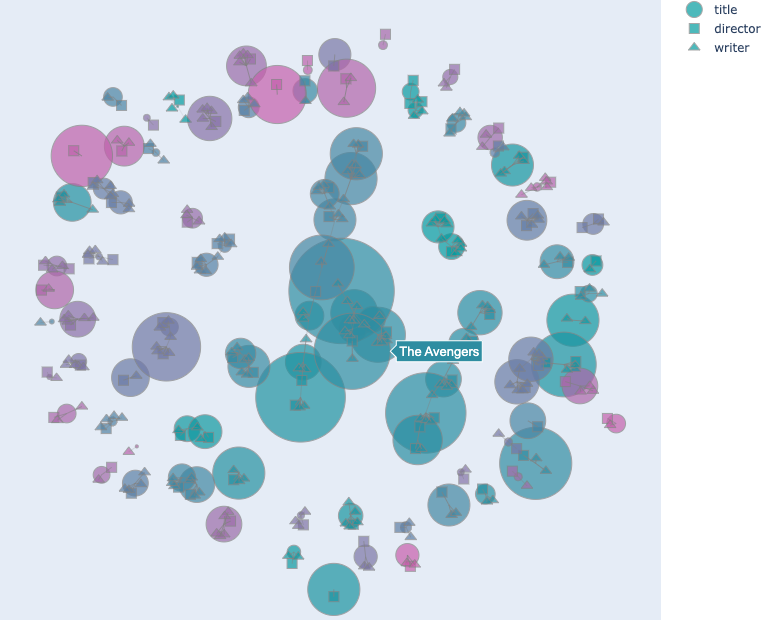
\includegraphics[width=\linewidth, height=0.9\linewidth]{figures/data_vis_1.png}
\tiny The entire network graph with user's mouse hovering over the node representing `Avengers'.
\end{minipage}\hfill
\begin{minipage}[t]{0.4\linewidth}
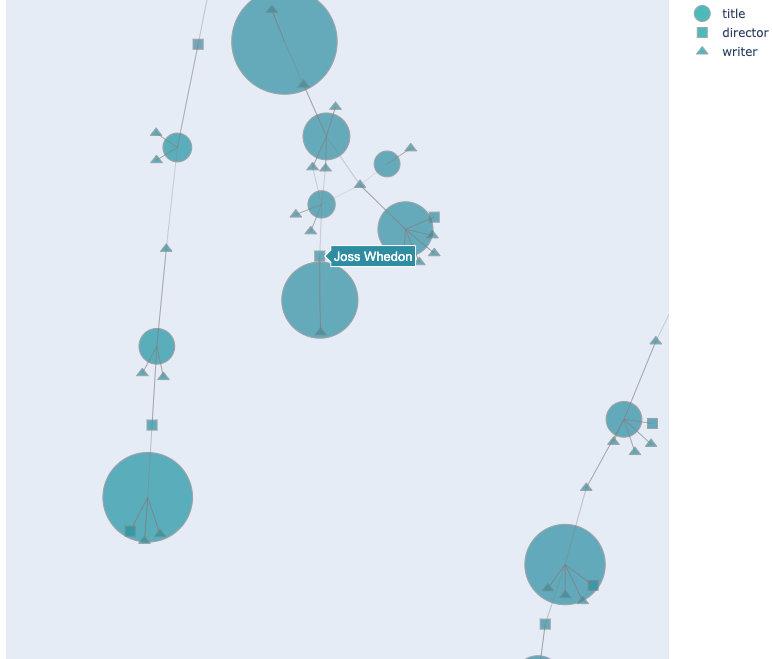
\includegraphics[trim={0 0 3cm 0}, clip, width=\linewidth, height=1\linewidth]{figures/data_vis_2.png}
\tiny Zoomed-in around the `Avengers' node with mouse hovering over the node of its director.
\end{minipage}
\tcbline
\parbox[t]{\linewidth}{\tiny\begin{alltt}
Human: I am a Hollywood producer. We are starting a new project for an adventure movie in 2023, we are currently making critical decisions on the choices of script writters and directors. For this purpose, I have gathered some historical data ranging from 1888 to 2022. I have an IMDb dataset that consists of the 4 following files:\\

\#\# title.basics.tsv.gz - Contains the following information for titles:\\
> tconst (string) - alphanumeric unique identifier of the title\\
> titleType (string) – the type/format of the title (e.g. movie, short, tvseries, tvepisode, video, etc)\\
> primaryTitle (string) – the more popular title / the title used by the filmmakers on promotional materials at the point of release\\
> originalTitle (string) - original title, in the original language\\
> startYear (YYYY) – represents the release year of a title. In the case of TV Series, it is the series start year\\
> endYear (YYYY) – TV Series end year. 'NA' for all other title types\\
> genres (string array) – includes up to three genres associated with the title\\
\#\# title.crew.tsv.gz – Contains the director and writer information for all the titles in IMDb. Fields include:\\
> tconst (string) - alphanumeric unique identifier of the title\\
> directors (array of nconsts) - director(s) of the given title\\
> writers (array of nconsts) – writer(s) of the given title\\
\#\# title.ratings.tsv.gz – Contains the IMDb rating and votes information for titles\\
> tconst (string) - alphanumeric unique identifier of the title\\
> averageRating – weighted average of all the individual user ratings\\
> numVotes - number of votes the title has received\\
\#\# name.basics.tsv.gz – Contains the following information for names:\\
> nconst (string) - alphanumeric unique identifier of the name/person\\
> primaryName (string)– name by which the person is most often credited\\
> primaryProfession (array of strings)– the top-3 professions of the person\\
> knownForTitles (array of tconsts) – titles the person is known for\\

I'd like to know the best way to visualize this dataset with a single plot, so that our decision process can be made easier. Of course, our goal is to make this the best rated movie ever. What do you think?\\
\\

AI: \hl{There are many possible ways to visualize this dataset, but one possible option is to use a network graph, where the nodes represent the titles, directors, writers, and actors, and the edges represent the relationships between them. The size and color of the nodes can be used to encode the average rating and the number of votes of the titles, or the popularity and reputation of the people. The thickness and opacity of the edges can be used to encode the frequency and strength of the collaborations between the nodes. This way, we can see the clusters and patterns of the most successful and influential titles and people in the film industry, and identify the potential candidates for our project.}
\\
\\
Human: I like the idea, but since this dataset is quite large, a network graph might look messy. Is there anyway to simplify it?
\\
\\
\end{alltt}}

\parbox[t]{\linewidth}{\tiny\begin{alltt}
AI:\hl{ Yes, there are some possible ways to simplify the network graph. For example, we could:\\
- Filter out the titles and people that are not relevant to our genre or time period of interest. For example, if we are making an adventure movie in 2023, we could exclude the titles that are not of the type movie or video, or that are not in the genre adventure, or that are released before 2010. We could also exclude the people that are not primarily involved in directing, writing, or acting, or that are deceased, or that have not worked on any relevant titles.\\
- Aggregate the nodes that belong to the same group or category, and use a representative node to show their collective attributes. For example, we could group the titles by their directors or writers, and use a single node to show the average rating and number of votes of their titles, as well as the names of the people in the group. We could also group the people by their primary profession, and use a single node to show their popularity and reputation, as well as the titles they are known for.\\
- Use a hierarchical or modular layout to organize the nodes by their level of similarity or connection. For example, we could use a force-directed layout to place the nodes that are more closely related or frequently collaborated closer together, and use a community detection algorithm to partition the nodes into subgroups based on their network structure. We could also use a tree or radial layout to show the nodes by their level of hierarchy or centrality, such as the most influential directors, writers, or actors at the center, and the less influential ones at the periphery.}

Human: I think the last suggestion makes a lot sense to me. Could you please implement it for me in Python?\\

AI:\hl{ Sure, here is a possible implementation of the network graph in Python, using the networkx, pandas, and plotly libraries. Note that this is not a fully functional code, and some parts are simplified or omitted for brevity. You will need to load and preprocess the dataset before running this code.}
\end{alltt}}
\vspace{-0.5cm}
\begin{minted}[breaklines, breaksymbol=, baselinestretch=1, fontsize=\tiny]{python}
# Import the libraries
import pandas as pd
import numpy as np
import networkx as nx
import plotly
import plotly.graph_objects as go

# Read the files
title_basics = pd.read_csv('title.basics.tsv.gz', sep='\t', na_values='NA')
title_crew = pd.read_csv('title.crew.tsv.gz', sep='\t', na_values='NA')
title_ratings = pd.read_csv('title.ratings.tsv.gz', sep='\t', na_values='NA')
name_basics = pd.read_csv('name.basics.tsv.gz', sep='\t', na_values='NA')

# Filter by titleType and genres
title_basics = title_basics.drop(columns=['endYear']).dropna()
title_basics = title_basics[title_basics['startYear']>=2010]
title_basics = title_basics[title_basics['titleType'] == 'movie']
title_basics = title_basics[title_basics['genres'].str.contains('Adventure')]

# Filter out NaN rows
name_basics = name_basics[name_basics['primaryProfession'].notnull() & name_basics['knownForTitles'].notnull()]

# Merge the files
title_data = title_basics.merge(title_crew, on='tconst')
title_data = title_data.merge(title_ratings, on='tconst')
title_data = title_data.merge(title_principals, on='tconst')
title_data = title_data.merge(name_basics, on='nconst')

# Create the graph
G = nx.Graph()
# Add the edges for the relationships between the nodes
# Use the thickness and opacity of the edges to encode the frequency and strength of the collaborations between the nodes
# Use some arbitrary functions to calculate the weight of the edges, such as count or mean
for index, row in title_data.iterrows():
  if not ('director' in row['category'] or 'writer' in row['category']):
     continue
  tconst = row['tconst']
  nconst = row['nconst']
  if not G.has_node(tconst):
      G.add_node(tconst, type='title', rating=row['averageRating'], votes=row['numVotes'], name=row['primaryTitle'])
      G.nodes[tconst]['size'] = 15 ** (row['averageRating'] / 5)
  if not G.has_node(nconst):
      G.add_node(nconst, type=row['category'], name=row['primaryName'], titles=row['knownForTitles'])
      G.nodes[nconst]['size'] = 10

  if G.has_edge(tconst, nconst):
    G.edges[tconst, nconst]['weight'] += 1
  else:
    G.add_edge(tconst, nconst, weight=1)
  G.edges[tconst, nconst]['width'] = G.nodes[tconst]['rating'] / 10
  G.edges[tconst, nconst]['alpha'] = G.edges[tconst, nconst]['weight'] / G.degree[nconst]


# Use a force-directed layout to place the nodes based on their connections
# Use a community detection algorithm to partition the nodes into subgroups based on their network structure
# Use different colors for the nodes based on their community
import community.community_louvain as community_louvain
import plotly.colors as pc
pos = nx.spring_layout(G)
partition = community_louvain.best_partition(G)
for node in G.nodes():
  G.nodes[node]['community'] = partition[node]

# Define a continuous color scale, for example, a diverging scale from red to blue
# This can be a list of colors, a string name of a built-in scale, or a plotly.colors.sequential or plotly.colors.diverging object
colorscale = pc.diverging.Tropic

# Define a function to get a color from the scale given a normalized value between 0 and 1
def get_color(value, scale=colorscale):
  # Use the plotly.colors.find_intermediate_color function to interpolate between the colors in the scale
  # This returns a color in the rgb format, e.g. 'rgb(255,0,0)'
  return pc.find_intermediate_color(scale[0], scale[-1], value, colortype='rgb')

# Define a function to get n colors from the scale, evenly spaced
def get_colors(n, scale=colorscale):
  # Use the numpy.linspace function to generate n values between 0 and 1
  import numpy as np
  values = np.linspace(0, 1, n)
  # Use the get_color function to map each value to a color
  colors = [get_color(v, scale) for v in values]
  return colors

colors = get_colors(len(set(partition.values())))


# Create the figure
fig = go.Figure()

# Draw the nodes by their type, size, and color
node_types = ['title', 'director', 'writer', 'actor']
node_shapes = ['circle', 'square', 'triangle-up', 'triangle-down']
# Draw the title nodes by their size and color
fig.add_trace(go.Scatter(x=[pos[node][0] for node in G.nodes() if G.nodes[node]['type'] == 'title'],
            y=[pos[node][1] for node in G.nodes() if G.nodes[node]['type'] == 'title'],
            mode='markers+text',
            name='title',
            marker=dict(symbol='circle',
                        size=[G.nodes[node]['size']  for node in G.nodes() if G.nodes[node]['type'] == 'title'],
                        color=[colors[G.nodes[node]['community']] for node in G.nodes() if G.nodes[node]['type'] == node_type],
                        line=dict(width=1, color='grey')),
            text=[G.nodes[node]['name'] for node in G.nodes() if G.nodes[node]['type'] == 'title'],
            textposition='top center',
            textfont=dict(size=8),
            hoverinfo='text',
            visible=False))

# Draw the edges by their width and opacity
for edge in G.edges():
  x0, y0 = pos[edge[0]]
  x1, y1 = pos[edge[1]]
  weight, width, alpha = G.edges[edge].values()
  fig.add_trace(go.Scatter(x=[x0, x1],
            y=[y0, y1],
            mode='lines',
            name='edge',
            opacity=alpha,
            line=dict(width=width,
                    color='grey'),
            hoverinfo='none')

# Add some labels and legends to the graph
fig.update_layout(title='',
            showlegend=True,
            margin=dict(l=20, r=20, t=30, b=20),
            autosize=True,
            width=800,
            height=800,
            hovermode='closest',
            xaxis=dict(showgrid=False, zeroline=False, showticklabels=False),
            yaxis=dict(showgrid=False, zeroline=False, showticklabels=False))
\end{minted}
\parbox[t]{1\linewidth}{\tiny\begin{alltt}
Human: Wow, this looks amazing! Maybe just one slight suggestion, I am seeing the edges showing up in the legends. As there are many of them, they eat up a lot space. Can you tell me where in the code I can make them disappear from the legend?
\\
\\
AI:\hl{ Sure, you can make the edges disappear from the legend by adding the argument showlegend=False to the go.Scatter trace that draws the edges.}
\\
\\
Human: Great, that works perfectly! One last thing, could you please remove all the title names and crew names? They clutter the plot. Instead, can you make them appear only when I move mouse onto them?
\\
\\
AI:\hl{ Sure, you can remove the text of title names by using the mode argument in the go.Scatter trace that draws the title nodes. For example, you can modify the code as follows:}
\end{alltt}}
\vspace{-.5cm}
\begin{minted}[breaklines, breaksymbol=, baselinestretch=1, fontsize=\tiny]{python}
# Draw the title nodes by their size and color
for i, node_type in enumerate(node_types):
  fig.add_trace(go.Scatter(x=[pos[node][0] for node in G.nodes() if G.nodes[node]['type'] == node_type],
           y=[pos[node][1] for node in G.nodes() if G.nodes[node]['type'] == node_type],
           mode='markers',
           name=node_type,
           marker=dict(symbol=node_shapes[i],
                       size=[G.nodes[node]['size']  for node in G.nodes() if G.nodes[node]['type'] == node_type],
                       color=[colors[G.nodes[node]['community']] for node in G.nodes() if G.nodes[node]['type'] == node_type],
                       line=dict(width=1, color='grey')),
           text=[G.nodes[node]['name'] for node in G.nodes() if G.nodes[node]['type'] == node_type],
           hoverinfo='text'))
\end{minted}

\end{tcolorbox}
%\caption{}
%\end{figure}

\subsection{More examples on visualization}
\begin{figure}[H]
\begin{AIbox}{\DV}
{\bf Prompt:} \begin{minted}[breaklines, breaksymbol=, baselinestretch=1, fontsize=\scriptsize]{html}
Can you write a pyplot code of the following 3D plot:
Dot plot x(t), y(t), z(t) = (1 - t)^0.5 * sin(5* pi * t), (1 - t)^0.5 *cos(5* pi * t), C*(1 - t) + 0.5(1 - C * C).
-I want to have 101 dots in the interval, from t = 0 to t = 1 with a gap 0.01. Name the dote d_1, d_2, ..., d_{101} where d1 is for t = 0 and d_{101} is for t = 101
-I want to animate the plot using the following way:
-The colors of the dots form a rainbow, and it's changing gradually every 0.2 seconds.
-The size of the i-th dot is proportional to i^1.5.
-Initially, C = 1, and C changes from 1 to 0 and then from 0 to 1 every 10 seconds.
-Add a horizontal plane in the plot, the z-axis is the current mean of those points.
\end{minted}
\vspace{-0.3cm}
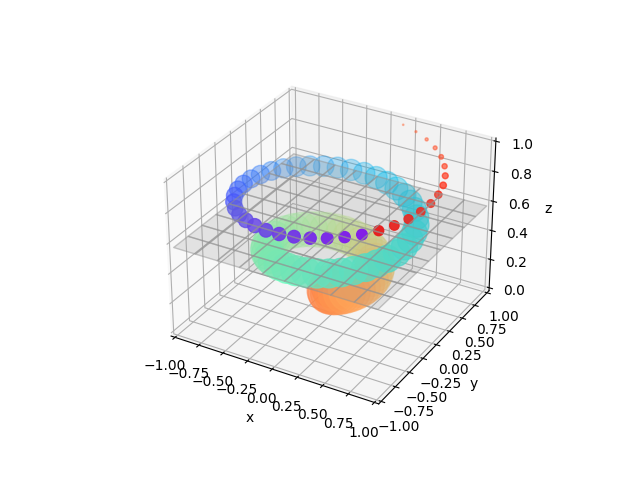
\includegraphics[trim={0 0 4cm 0}, width=0.4\linewidth]{figures/p4.png}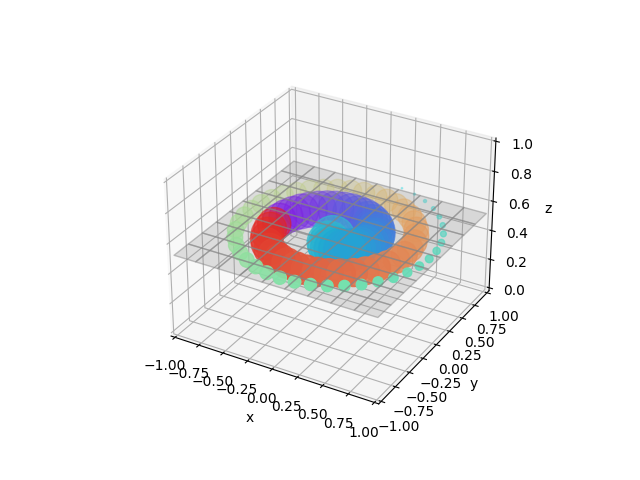
\includegraphics[trim={0 0 4cm 0}, width=0.4\linewidth]{figures/p3.png}
\end{AIbox}
\caption{An impressive visualization created by \DV \ from vague human instructions. \DV \ successfully interprets what it means by ``colors form a rainbow and changing gradually every 0.2 seconds'', \DV \ also sets all other details in the plot exactly as instructed, \emph{including the timings}.}
\label{fig:plot-2}
\end{figure}

%\newpage
\subsection{Example for 2D HTML game development}

\begin{AIbox}{\DV}
{\bf\scriptsize Prompt:} \vspace{-5px}
\begin{minted}[breaklines, breaksymbol=, baselinestretch=1, fontsize=\scriptsize]{html}
Can you write a 2D tank war game in HTML with Javascript? You can use a square to represent the tank, a triangle to represent the front of the tank, and use a ball to represent the bullet shell. I want to generate some random walls at the beginning of the game, and when the shell hits the wall, the wall disappears. The player wins the game if he destroys all enemy tanks. If the player's tank gets hit, then he loses the game. The player uses WASD to control the moves of the tank, and uses space to fire a shell. The enemy tanks are moving randomly and fire randomly.
\end{minted}
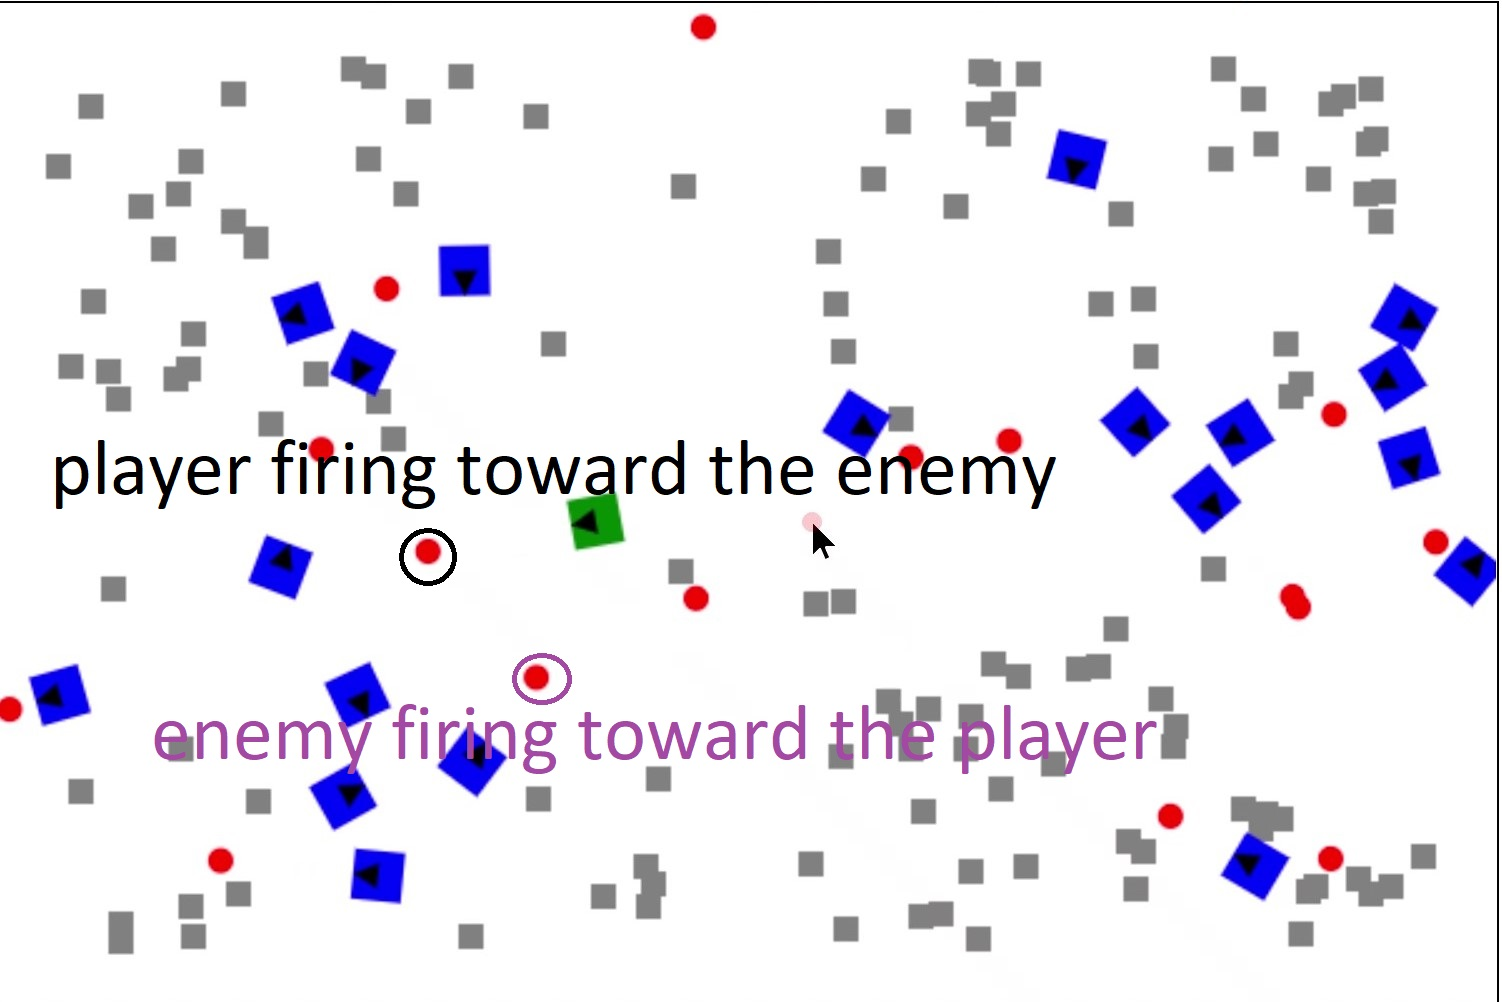
\includegraphics[height=0.32\linewidth]{figures/t01.jpg} \hfill 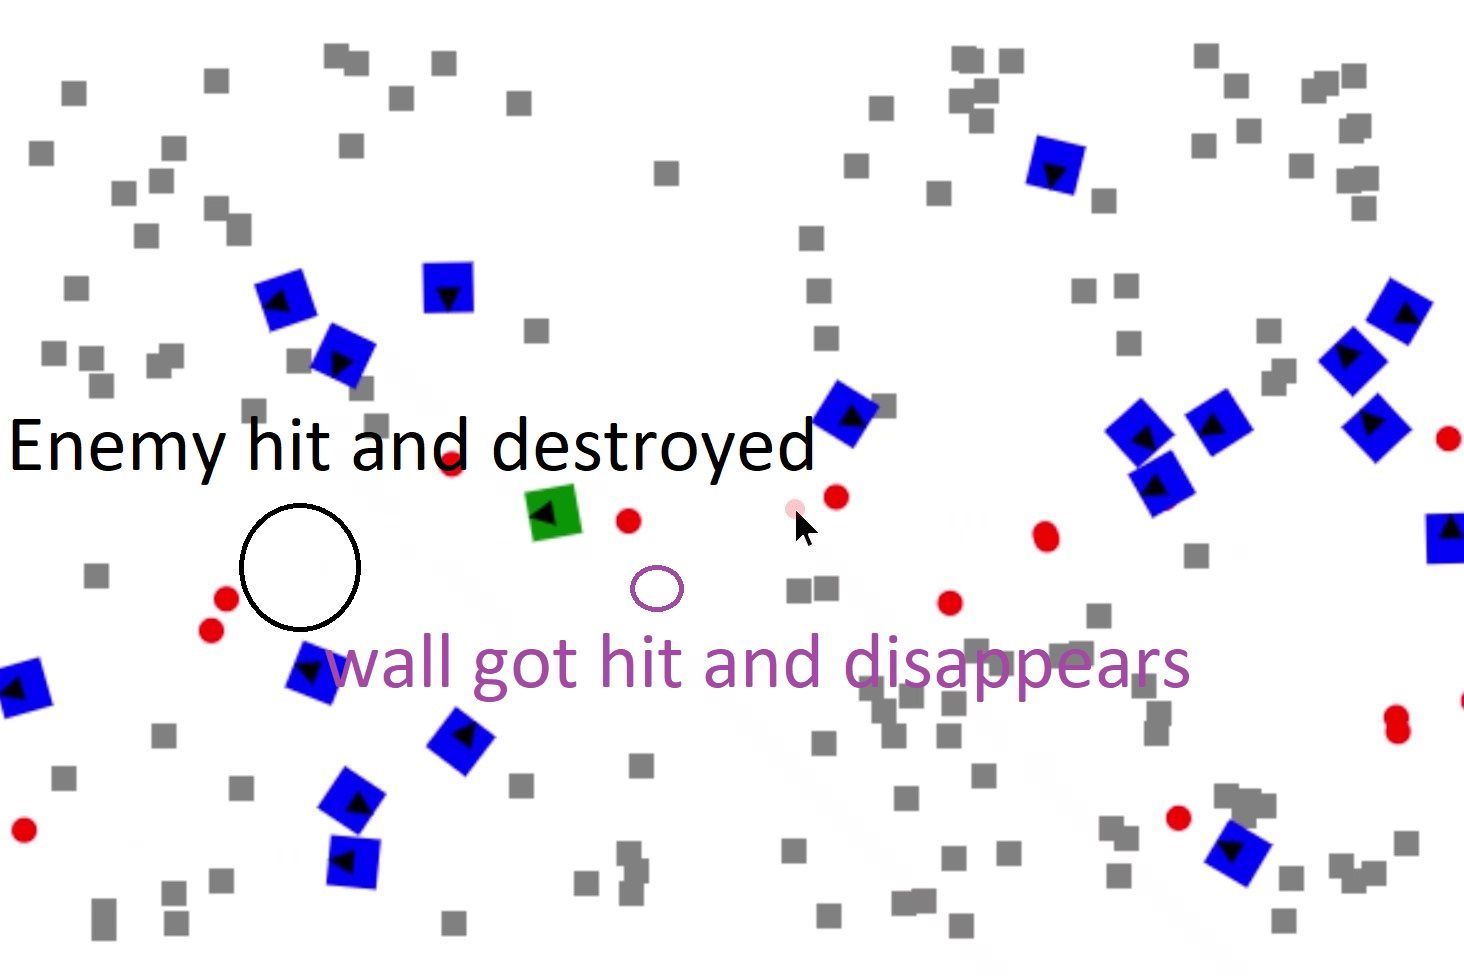
\includegraphics[height=0.32\linewidth]{figures/t02.jpg}
\end{AIbox}

Above, we ask \DV\ to write a 2D tank war game in HTML with JavaScript, using a vague level of specification.
The game involves complex logic and state management for the enemy, player, shell, and wall objects, as well as logic for collisions.
Again, \DV{} produces a fully functioning game, even adding ``common sense'' unspecified details such as ``shells should disappear after they hit a wall''. It is also able to edit the game according to user requests.  In contrast, ChatGPT not only refuses to create the game, but produces code for a square and a triangle that \emph{does not} move according the WASD keys. It does not move at all, it only points down when `d' is pressed and up when `a' is pressed (and even that is wrong, as `w' should point up, and `s' down).

\subsection{Example for graphical user interface programming}
 
GUI programming, or graphical user interface programming, is the process of designing and implementing software applications that interact with users through visual elements, such as windows, buttons, menus, icons, and dialogs. GUI programming is important because it can enhance the usability, accessibility, and attractiveness of software, as well as facilitate complex tasks and data visualization. However, GUI programming is also difficult, as it requires a combination of skills and knowledge, such as graphic design, user interface design, event-driven programming, platform-specific libraries and frameworks, and testing and debugging. We demonstrate that \DV\ is also an expert in GUI programming, knowing how to create an accurate layout and handle complicated input events.




%\begin{tcbraster}[raster columns=1, raster rows=2, size=small, raster halign=center, raster valign=center]
\begin{figure}[H]
\begin{AIbox}{\DV}
\begin{minted}[breaklines, breaksymbol=, baselinestretch=1, fontsize=\tiny]{html}
Can you write a python GUI with the following properties:
(1). The GUI contains three text fields, one single line (editable) on top, and one large multi-line text field (editable)in the middle, one single line (non-editable) on the bottom.
-- I want the multi-line text field to highlight things like a latex compiler. 
(2). It also contains three buttons: Submit and Cancel and Load.
(3). When hitting the submit button, the button becomes unhittable, and 
-- The program parses the input in the first text field, the input should be of form "-Ai=Bi" for a i = 1, 2, 3 , ..., separated by ; . The program creates a dictionary called input_parameters with keys of those Ai and values those Bi.
--The program parses the second large text field, and store it as a string called input_text.  
-- The program calls a function called query_model (you don't need to write it) with input_text and input_parameters as inputs.
--The program wait for the query_model to run, the query_model will return two strings: result_str, debug_info.
--The program will fill the bottom text field with the debug_info, and append the result_str to the text in the multi-line text field. 
-The program keeps running query_model again and again, until either of the following:
-(a). the returned result_str has length <= 10.
-(b). The cancel button is hitted. 
-After the model stops, it saves the text to ./data folder, with name text_XY, where X is the current time, Y is a k-word summarization of the text.
\end{minted}
\begin{comment}
\begin{minted}[breaklines, breaksymbol=, baselinestretch=1, fontsize=\tiny]{python}
def submit():
    text = text_entry.get("1.0", tk.END)
    # Disable the submit button and enable the cancel button
    submit_button.config(state=tk.DISABLED)
    cancel_button.config(state=tk.NORMAL)
    # Get the input parameters and text from the text fields
    input_str = parameter_entry.get()
    input_text = text_entry.get("1.0", tk.END)
    # Parse the input parameters into a dictionary
    input_parameters = parse_parameters(input_str)
    # Create a global thread object and assign it to the query_model function with the input parameters and text
    global thread
    global stop_flag
    stop_flag = False
    thread = threading.Thread(target=query_model, args=(input_text, input_parameters))
    # Start the thread
    thread.start()
def cancel():
    # Enable the submit button and disable the cancel button
    submit_button.config(state=tk.NORMAL)
    cancel_button.config(state=tk.DISABLED)
    # Set the global flag to True
    global stop_flag
    stop_flag = True
In query model:
    global stop_flag
    if not stop_flag:
        # Update the GUI with the results and debug info
        update_gui(result_str, debug_info, cc = cc)
    else:
        # Reset the global flag to False and save text
        save_text()
        stop_flag = False
In update_gui():
    if len(result_str) <= 10 or cancel_button["state"] == tk.DISABLED:
        # Enable the submit button and disable the cancel button
        submit_button.config(state=tk.NORMAL)
        cancel_button.config(state=tk.DISABLED)
        save_text()
    else:
        # Run the query_model function again with the updated text and parameters
        input_text = text_entry.get("1.0", tk.END)
        input_parameters = parse_parameters(parameter_entry.get())
        global thread
        thread = threading.Thread(target=query_model, args=(input_text, input_parameters))
        thread.start()
\end{minted}
\end{comment}
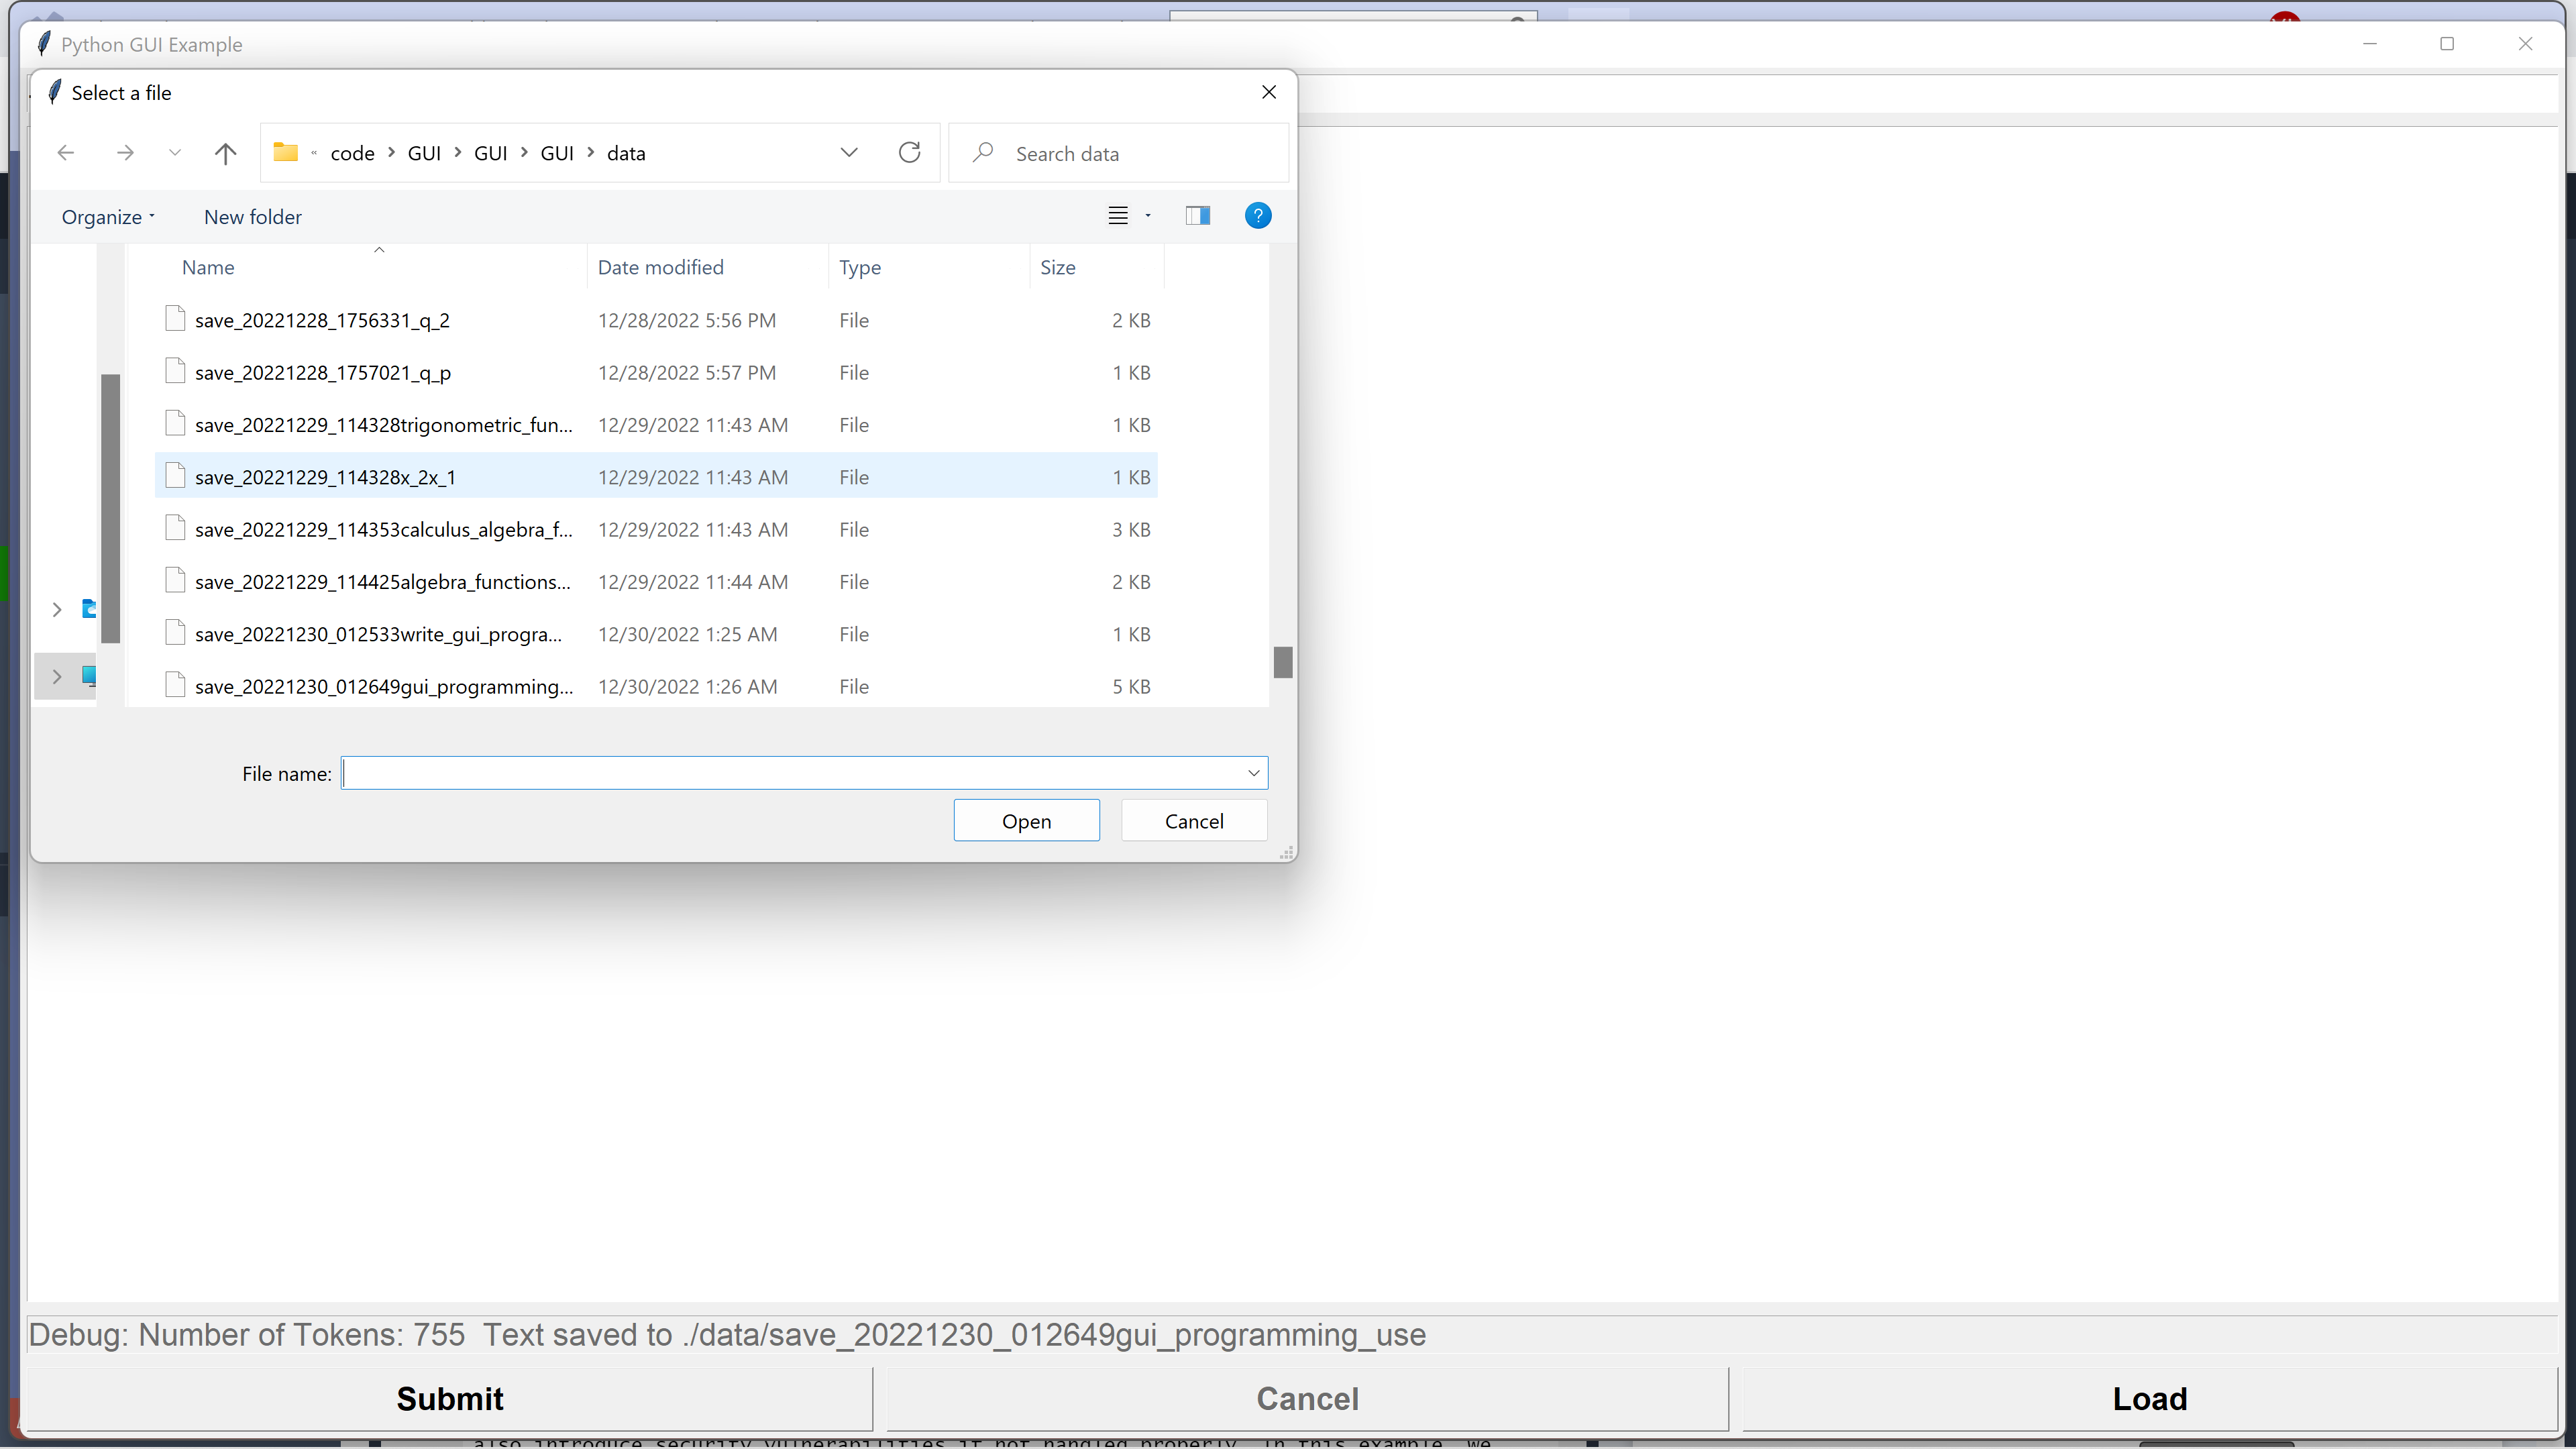
\includegraphics[width=0.45\linewidth]{figures/s1.png} \hfill 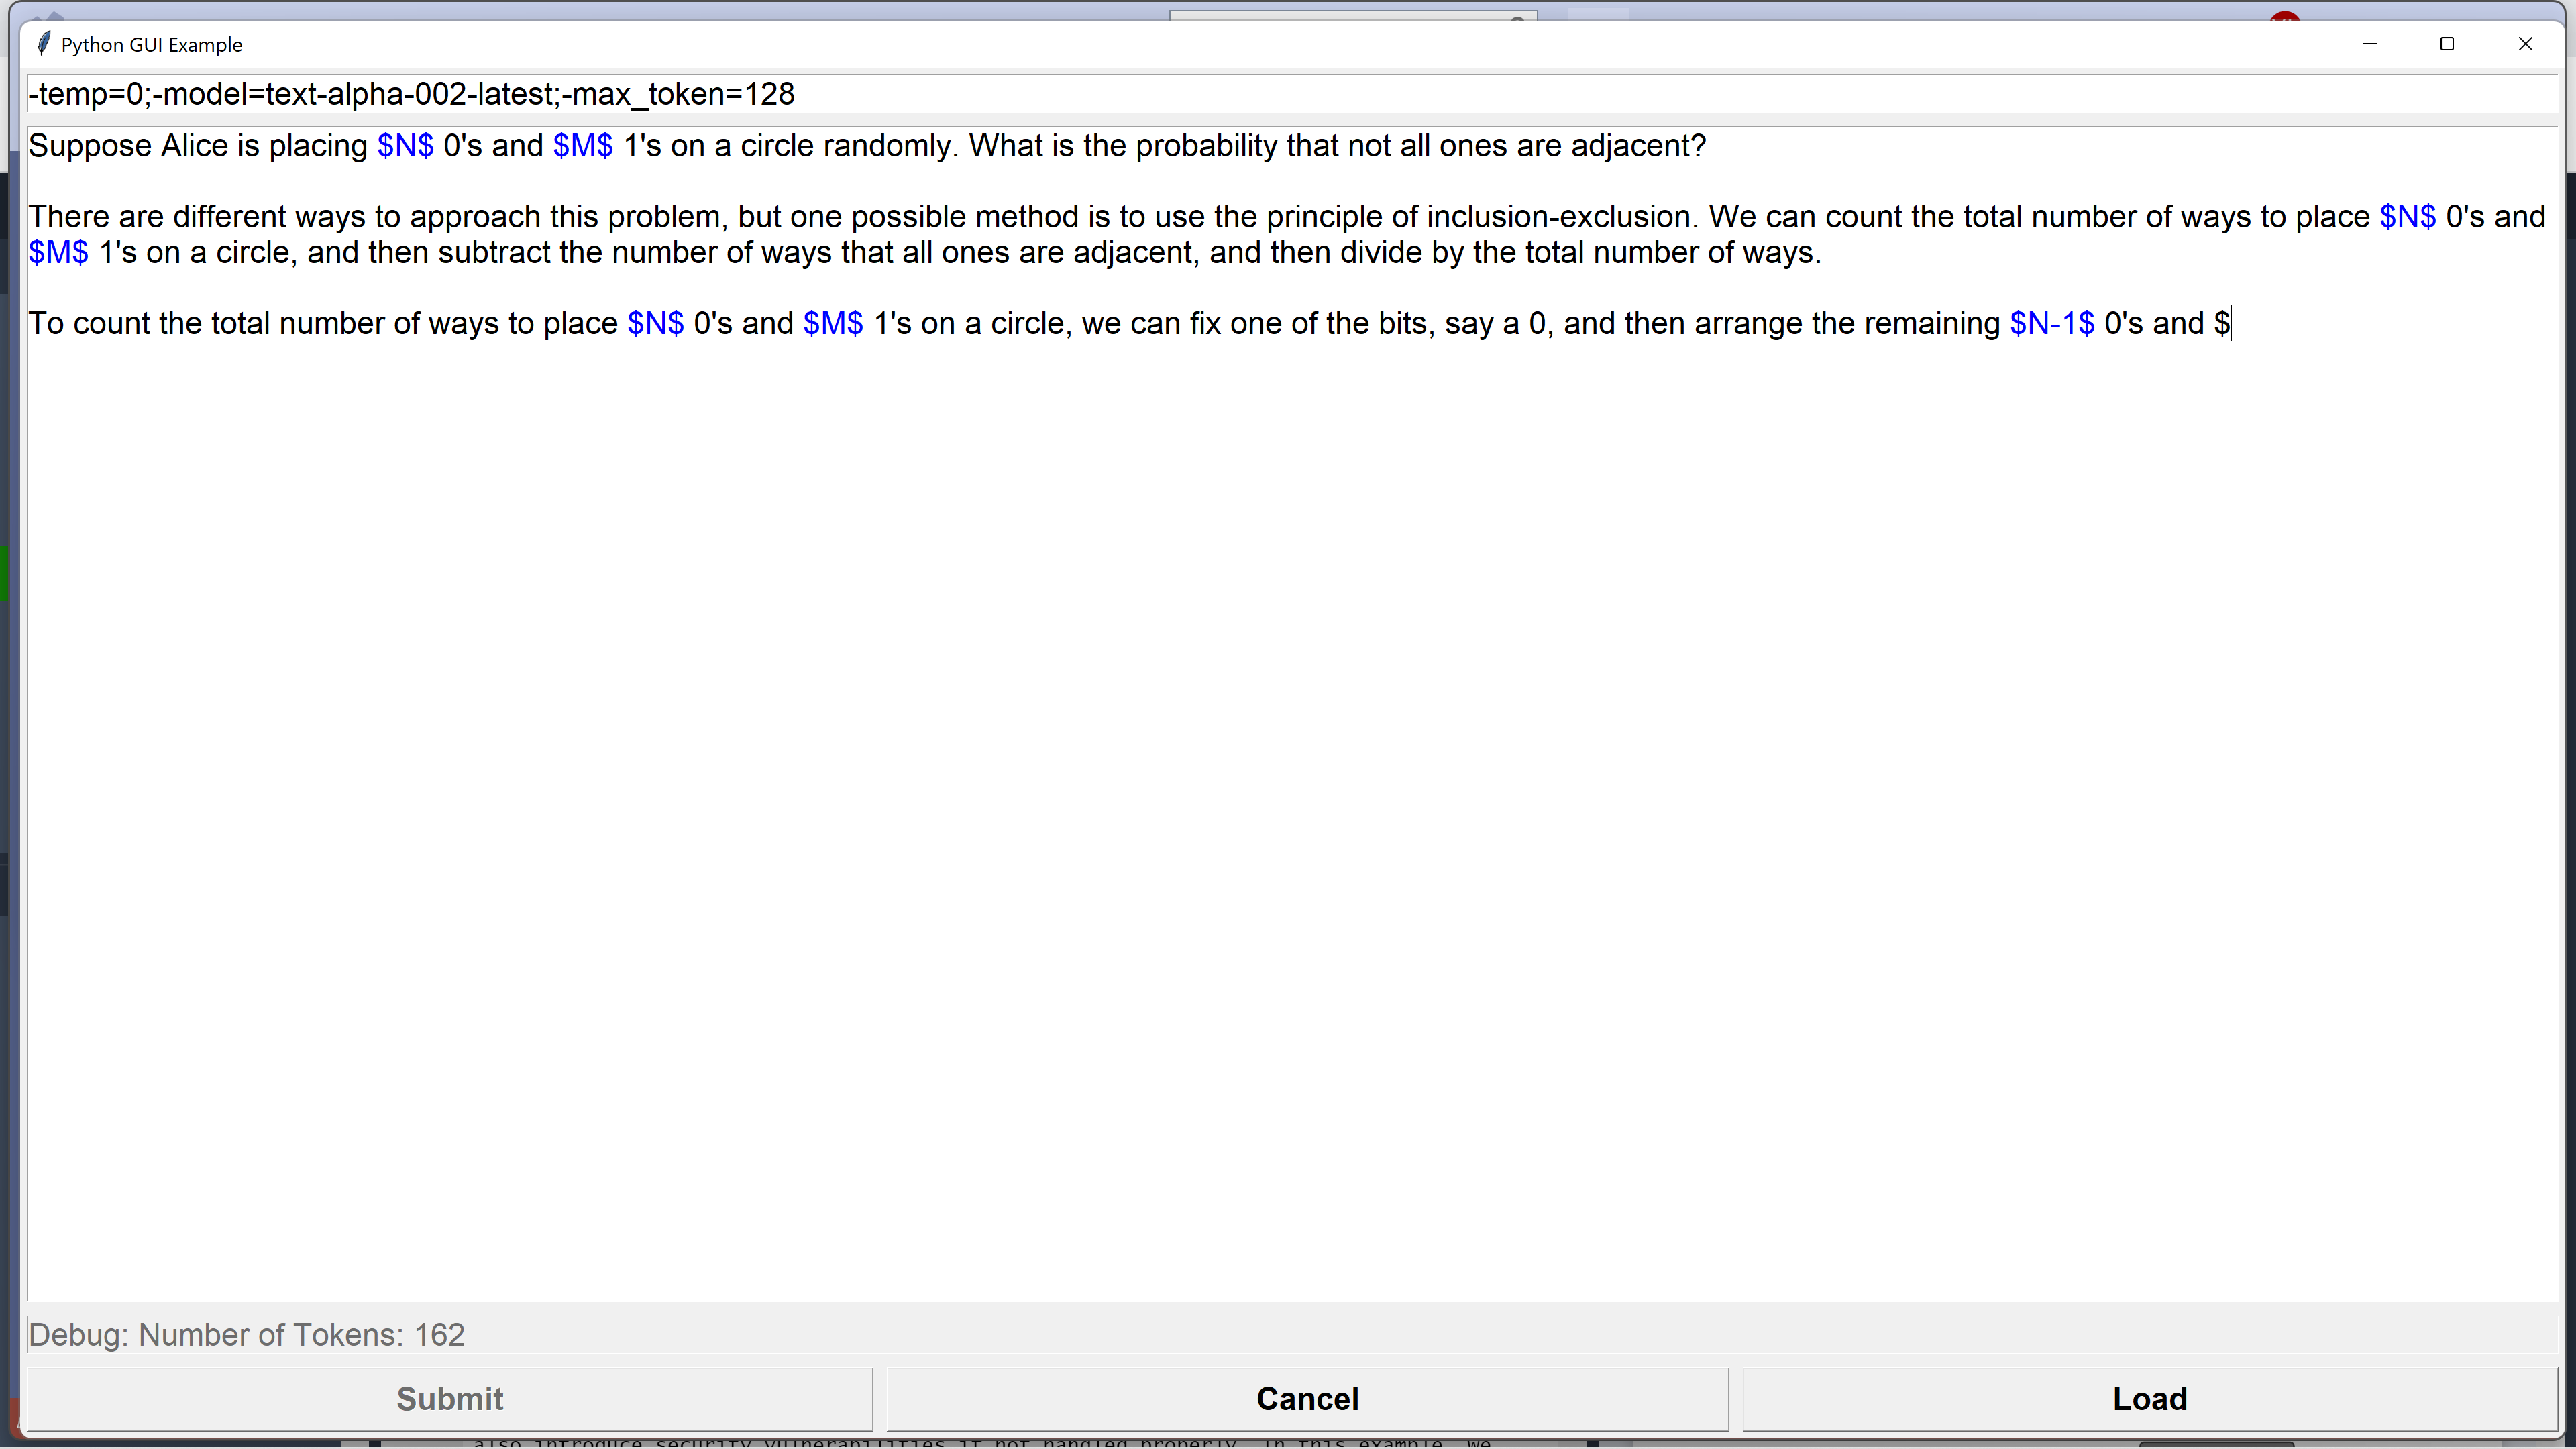
\includegraphics[width=0.45\linewidth]{figures/s2.png}
\end{AIbox}
\caption{\DV writes the program that generates a GUI for query\_model based on a prompt.}
\end{figure}
\DV analyzes the prompt and extracts the relevant details, such as the layout, the widgets, the labels, and the actions. It creates a separate thread for query\_model to avoid blocking the GUI while it runs, and it sets flags to terminate the thread if the user cancels the operation. It uses a regular expression to identify and highlight the expressions enclosed by \$ symbols, as the latex compiler does. It also uses the nltk package to produce a summary of the text after the query\_model finishes. Furthermore, it infers from common sense that the load button should allow the user to browse and select a file to load into the text\_entry, even though the prompt does not specify this functionality.





We test \DV's zero-shot GUI programming ability again by asking it a quite challenging task: Creating a drawing panel and keeping track of the list of previously drawn objects:



\begin{figure}[H]
\begin{AIbox}{\DV}
\begin{minted}[breaklines, breaksymbol=, baselinestretch=1, fontsize=\tiny]{html}
I want a python drawer GUI in tkinter.

I want to have a list of buttons in the bottom, they are:

Save/load images (png, jepg, jpg etc)

-Draw lines
-Draw arrow
-Draw curved arrow
-Draw Ellipse (only the edge)
-Draw rectangle (only the edge)
-Enter (multiple lines) Text (with the option to select text size, color and font)
-Select color, width
-Delete

I need  a scroll bar on the right, after I draw one object (**such as a line, an arrow , a text field**), it lists the object in the field. When I select the object in the list, it should highlight it. After that when I press delete, it should delete the corresponding object in the drawing that I selected. 

\end{minted}
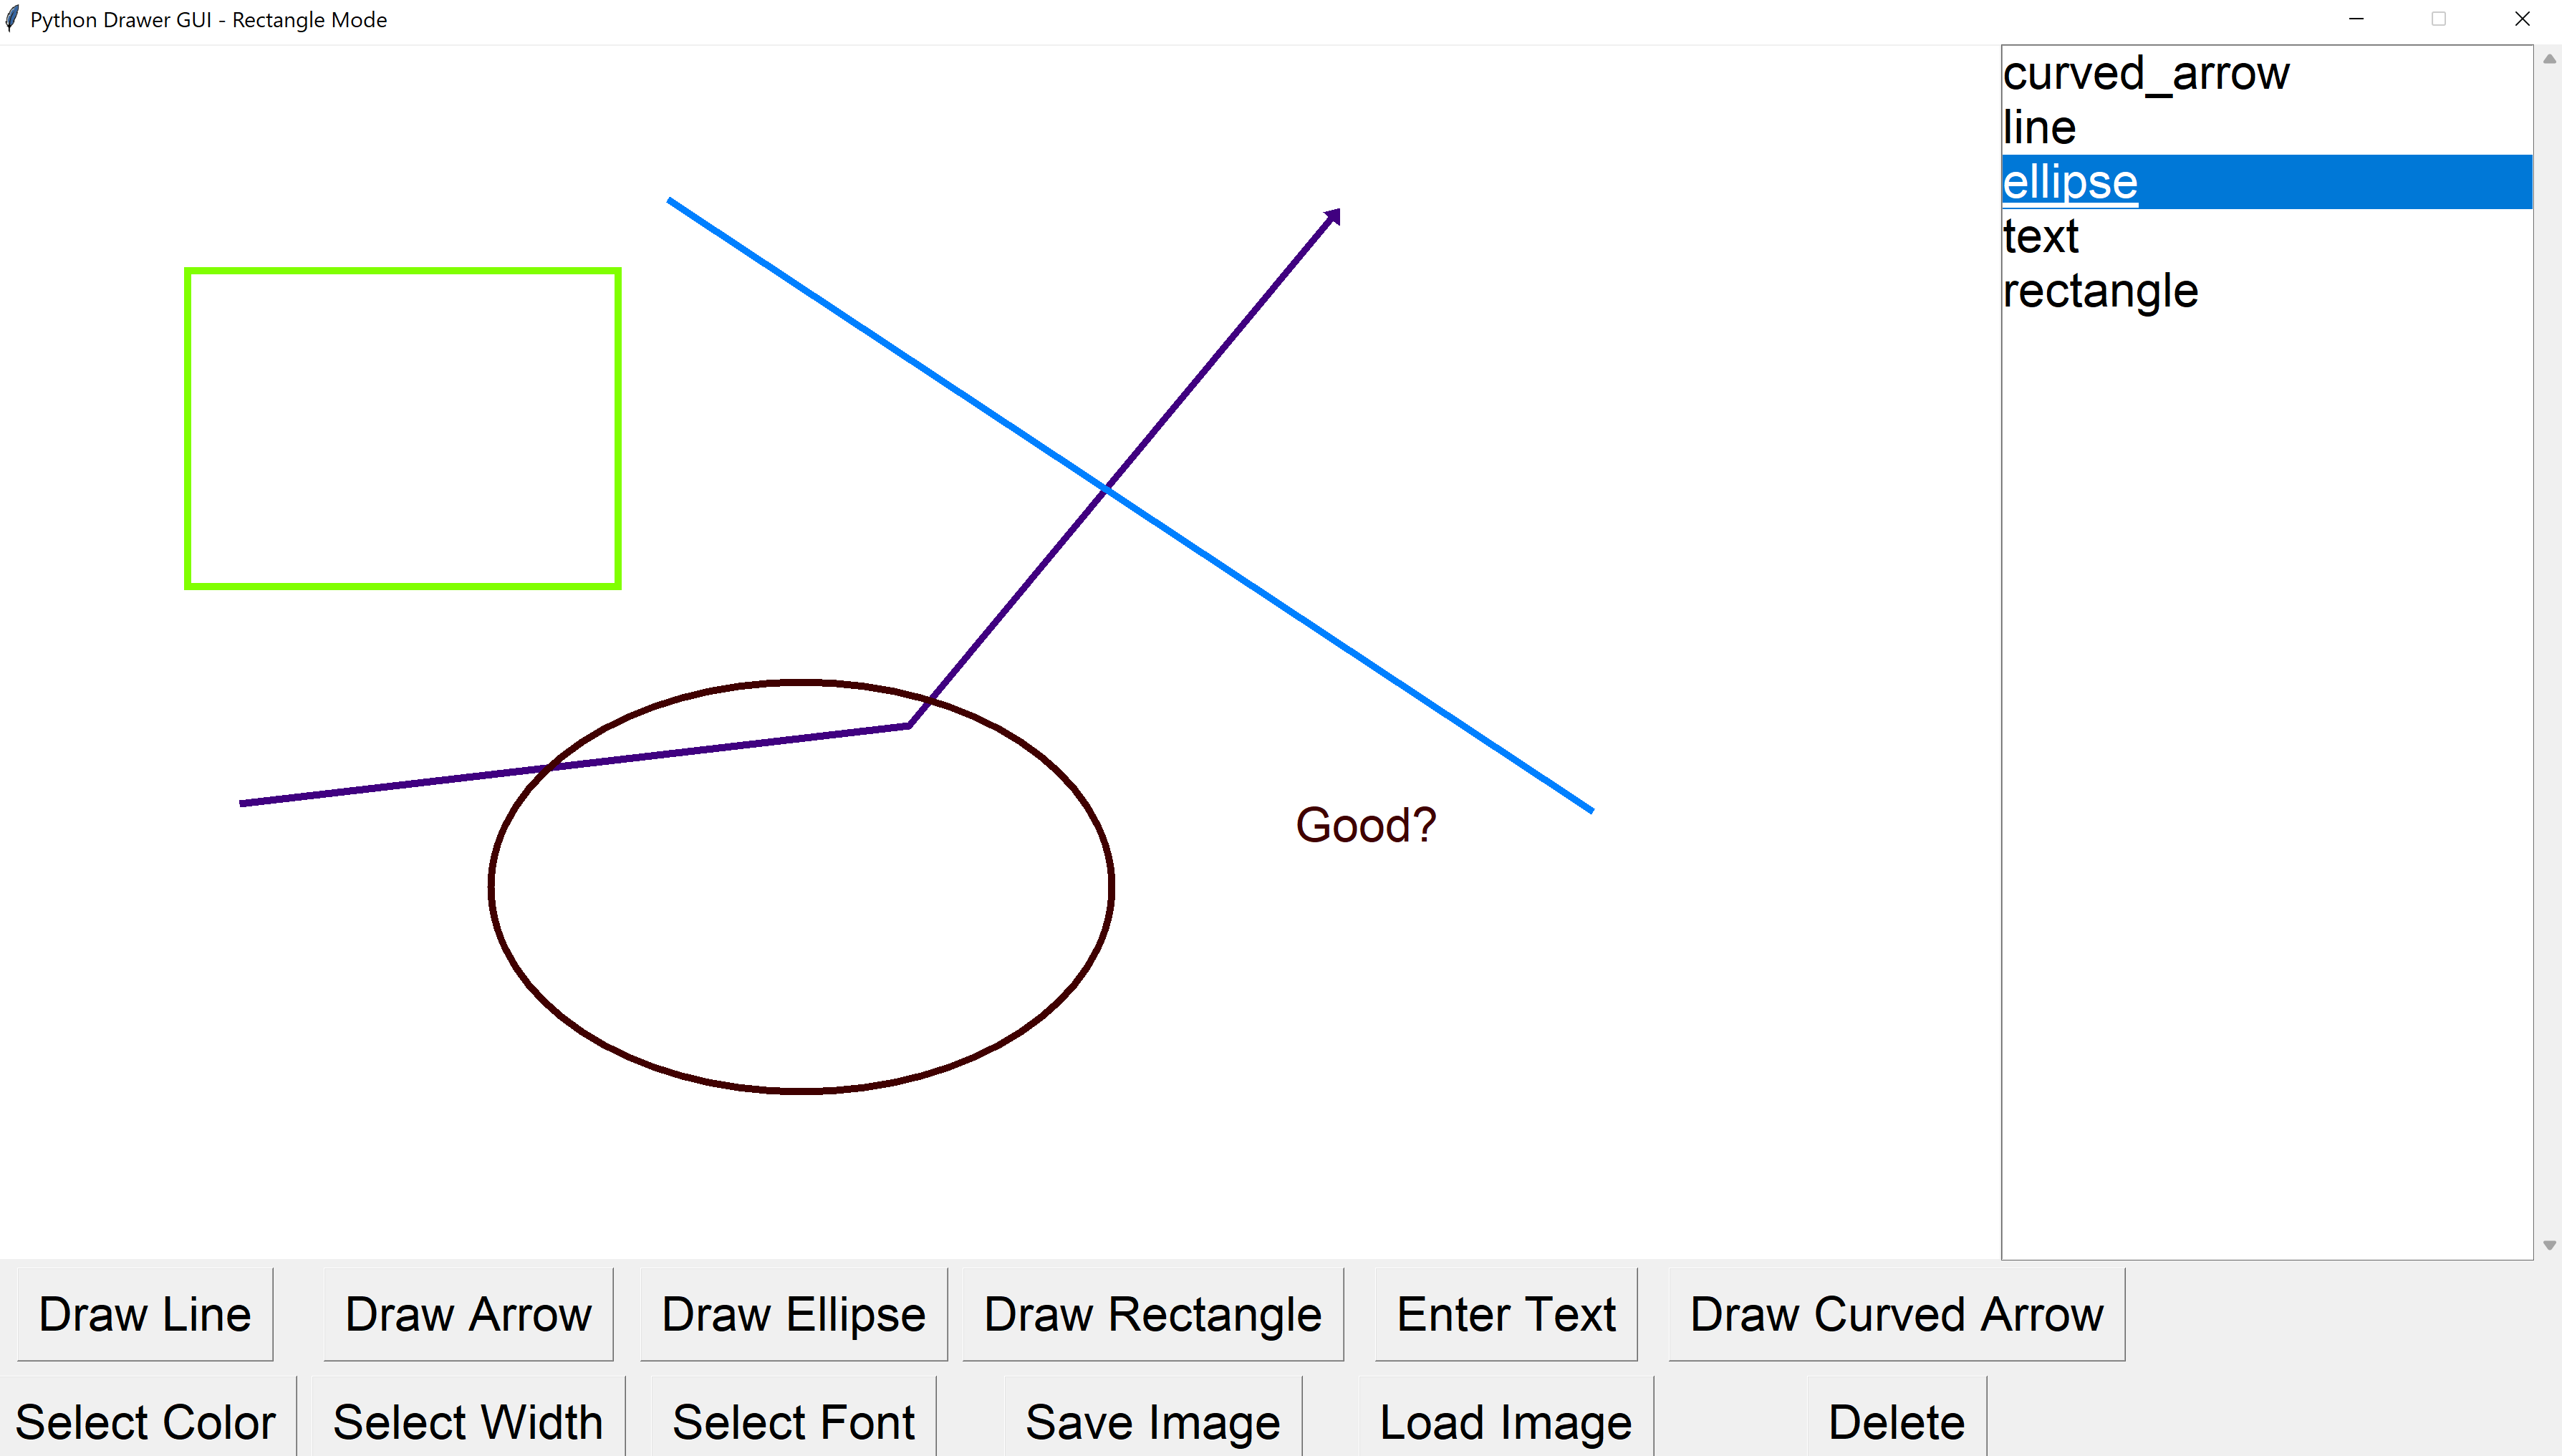
\includegraphics[width=0.45\linewidth]{figures/g4.png} \hfill 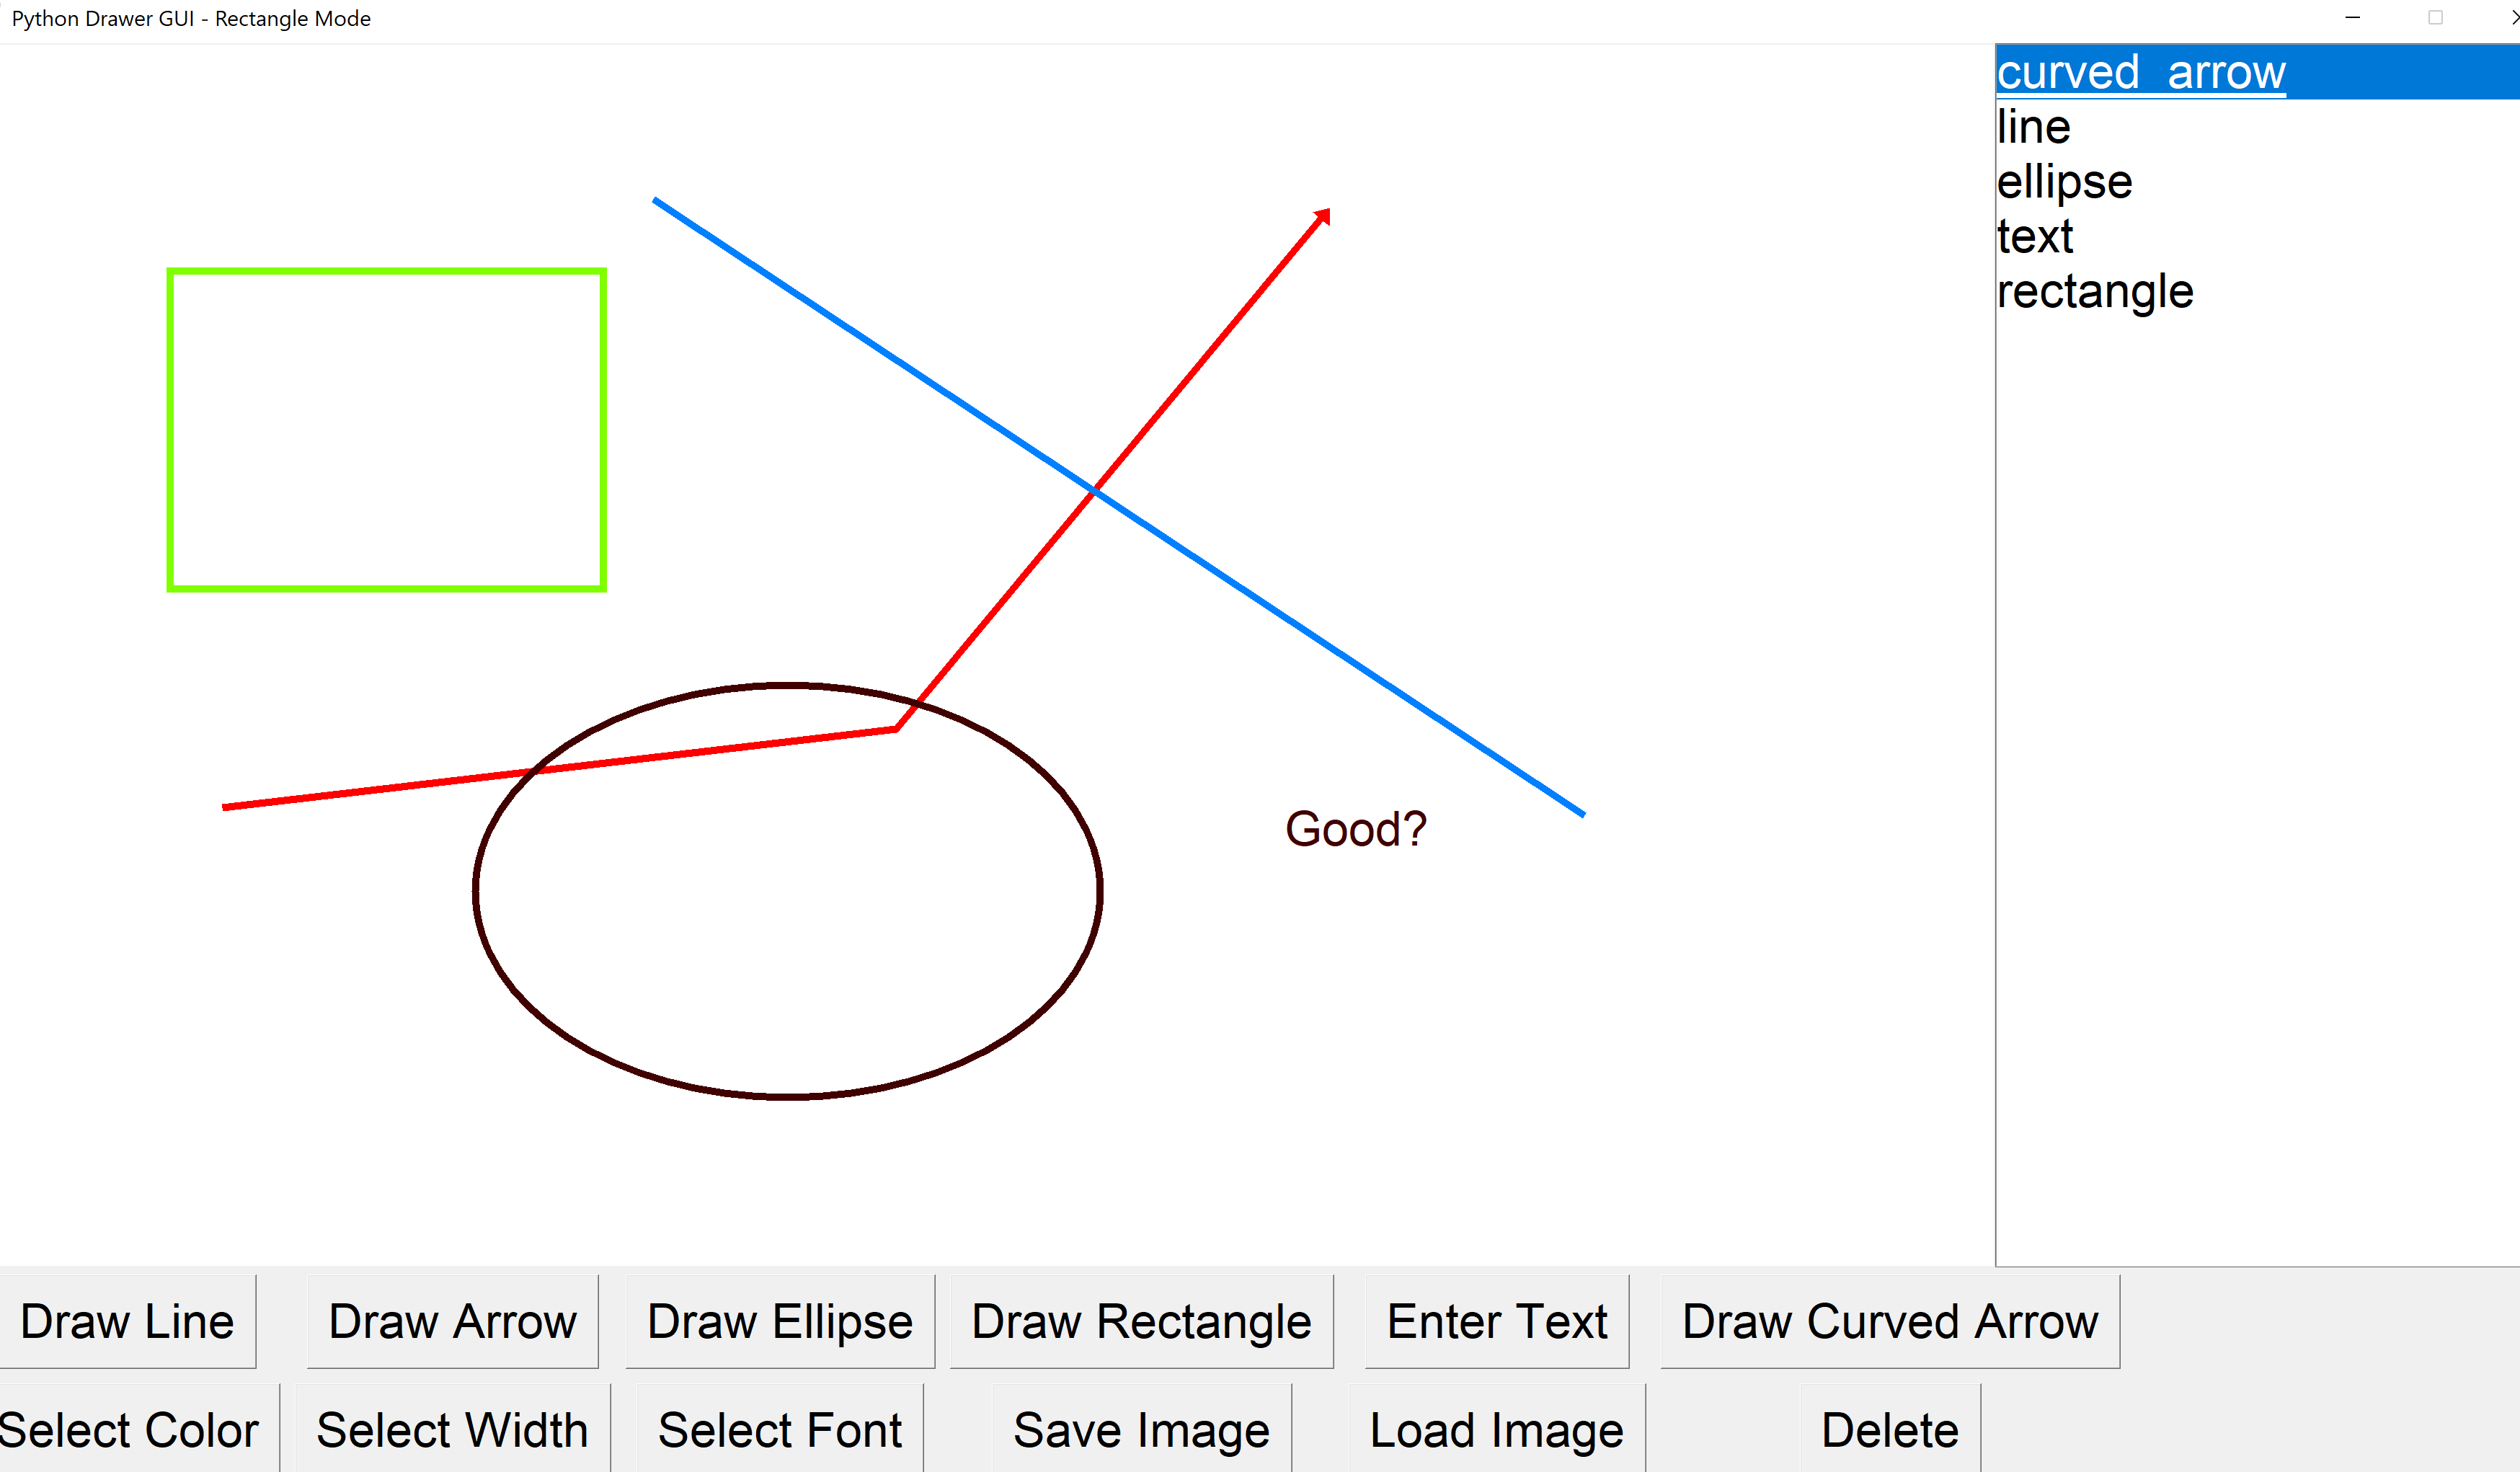
\includegraphics[width=0.45\linewidth]{figures/g20.png}
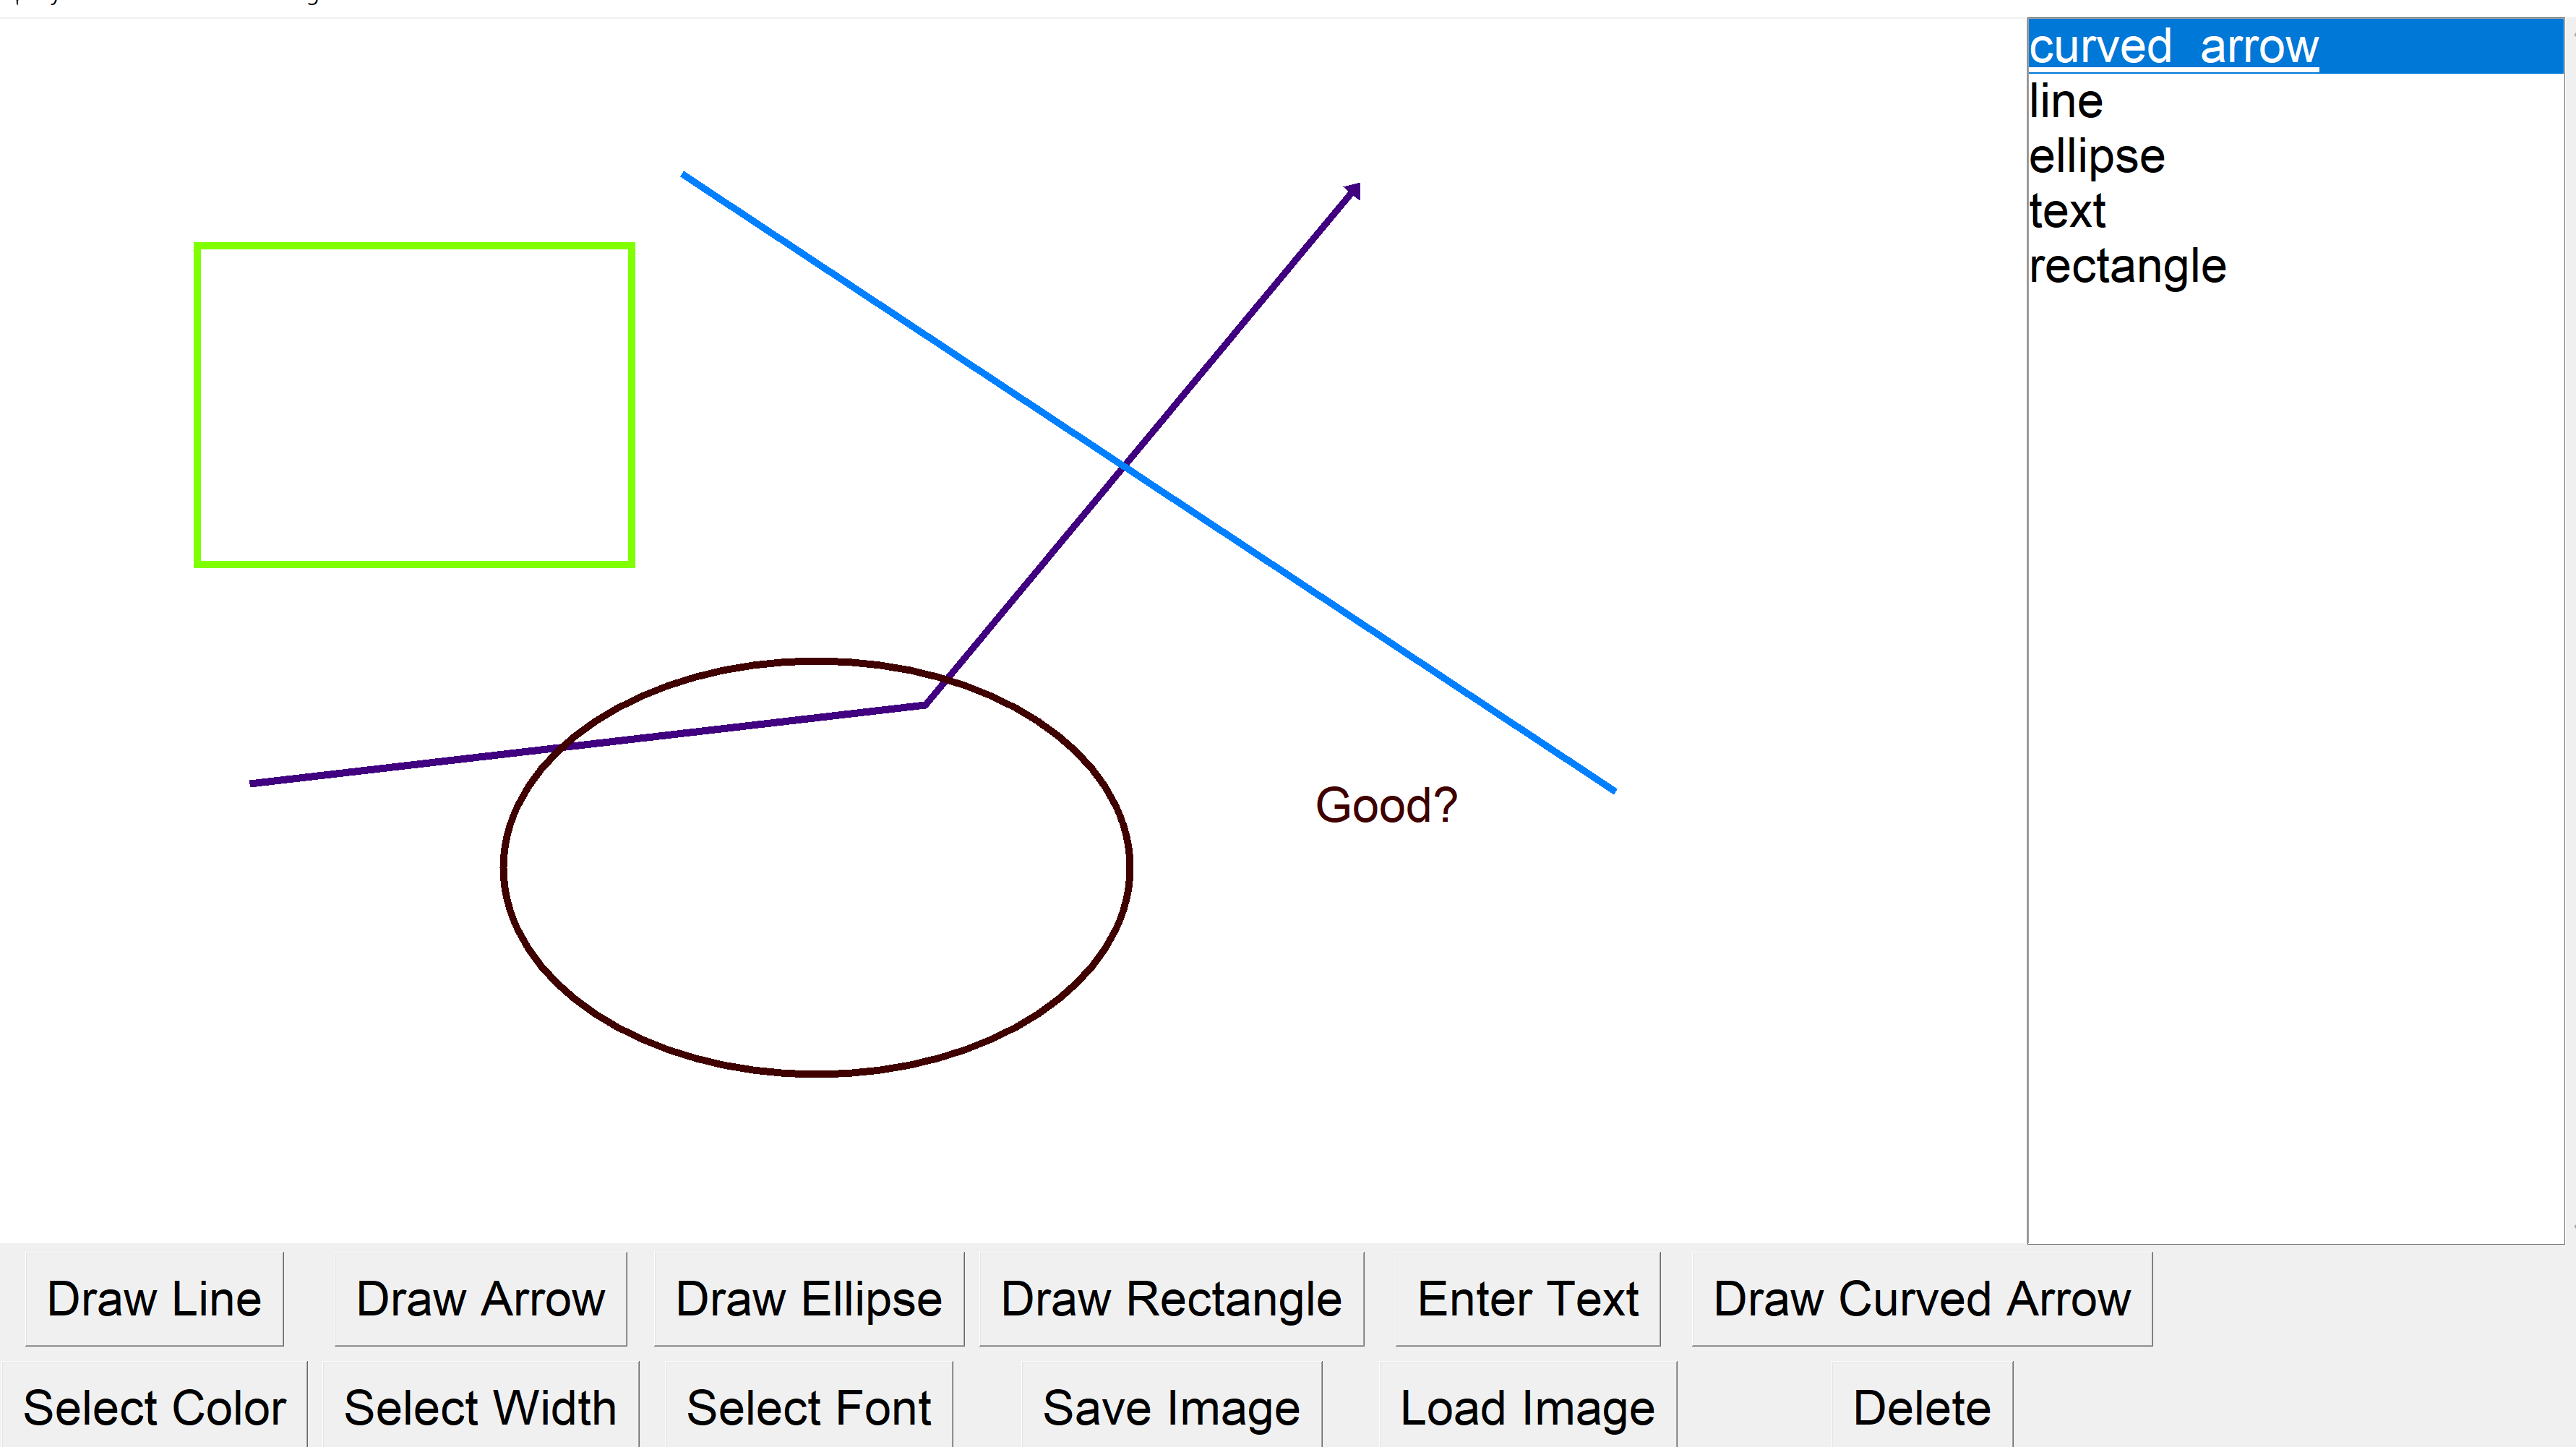
\includegraphics[width=0.45\linewidth]{figures/g3.png} \hfill 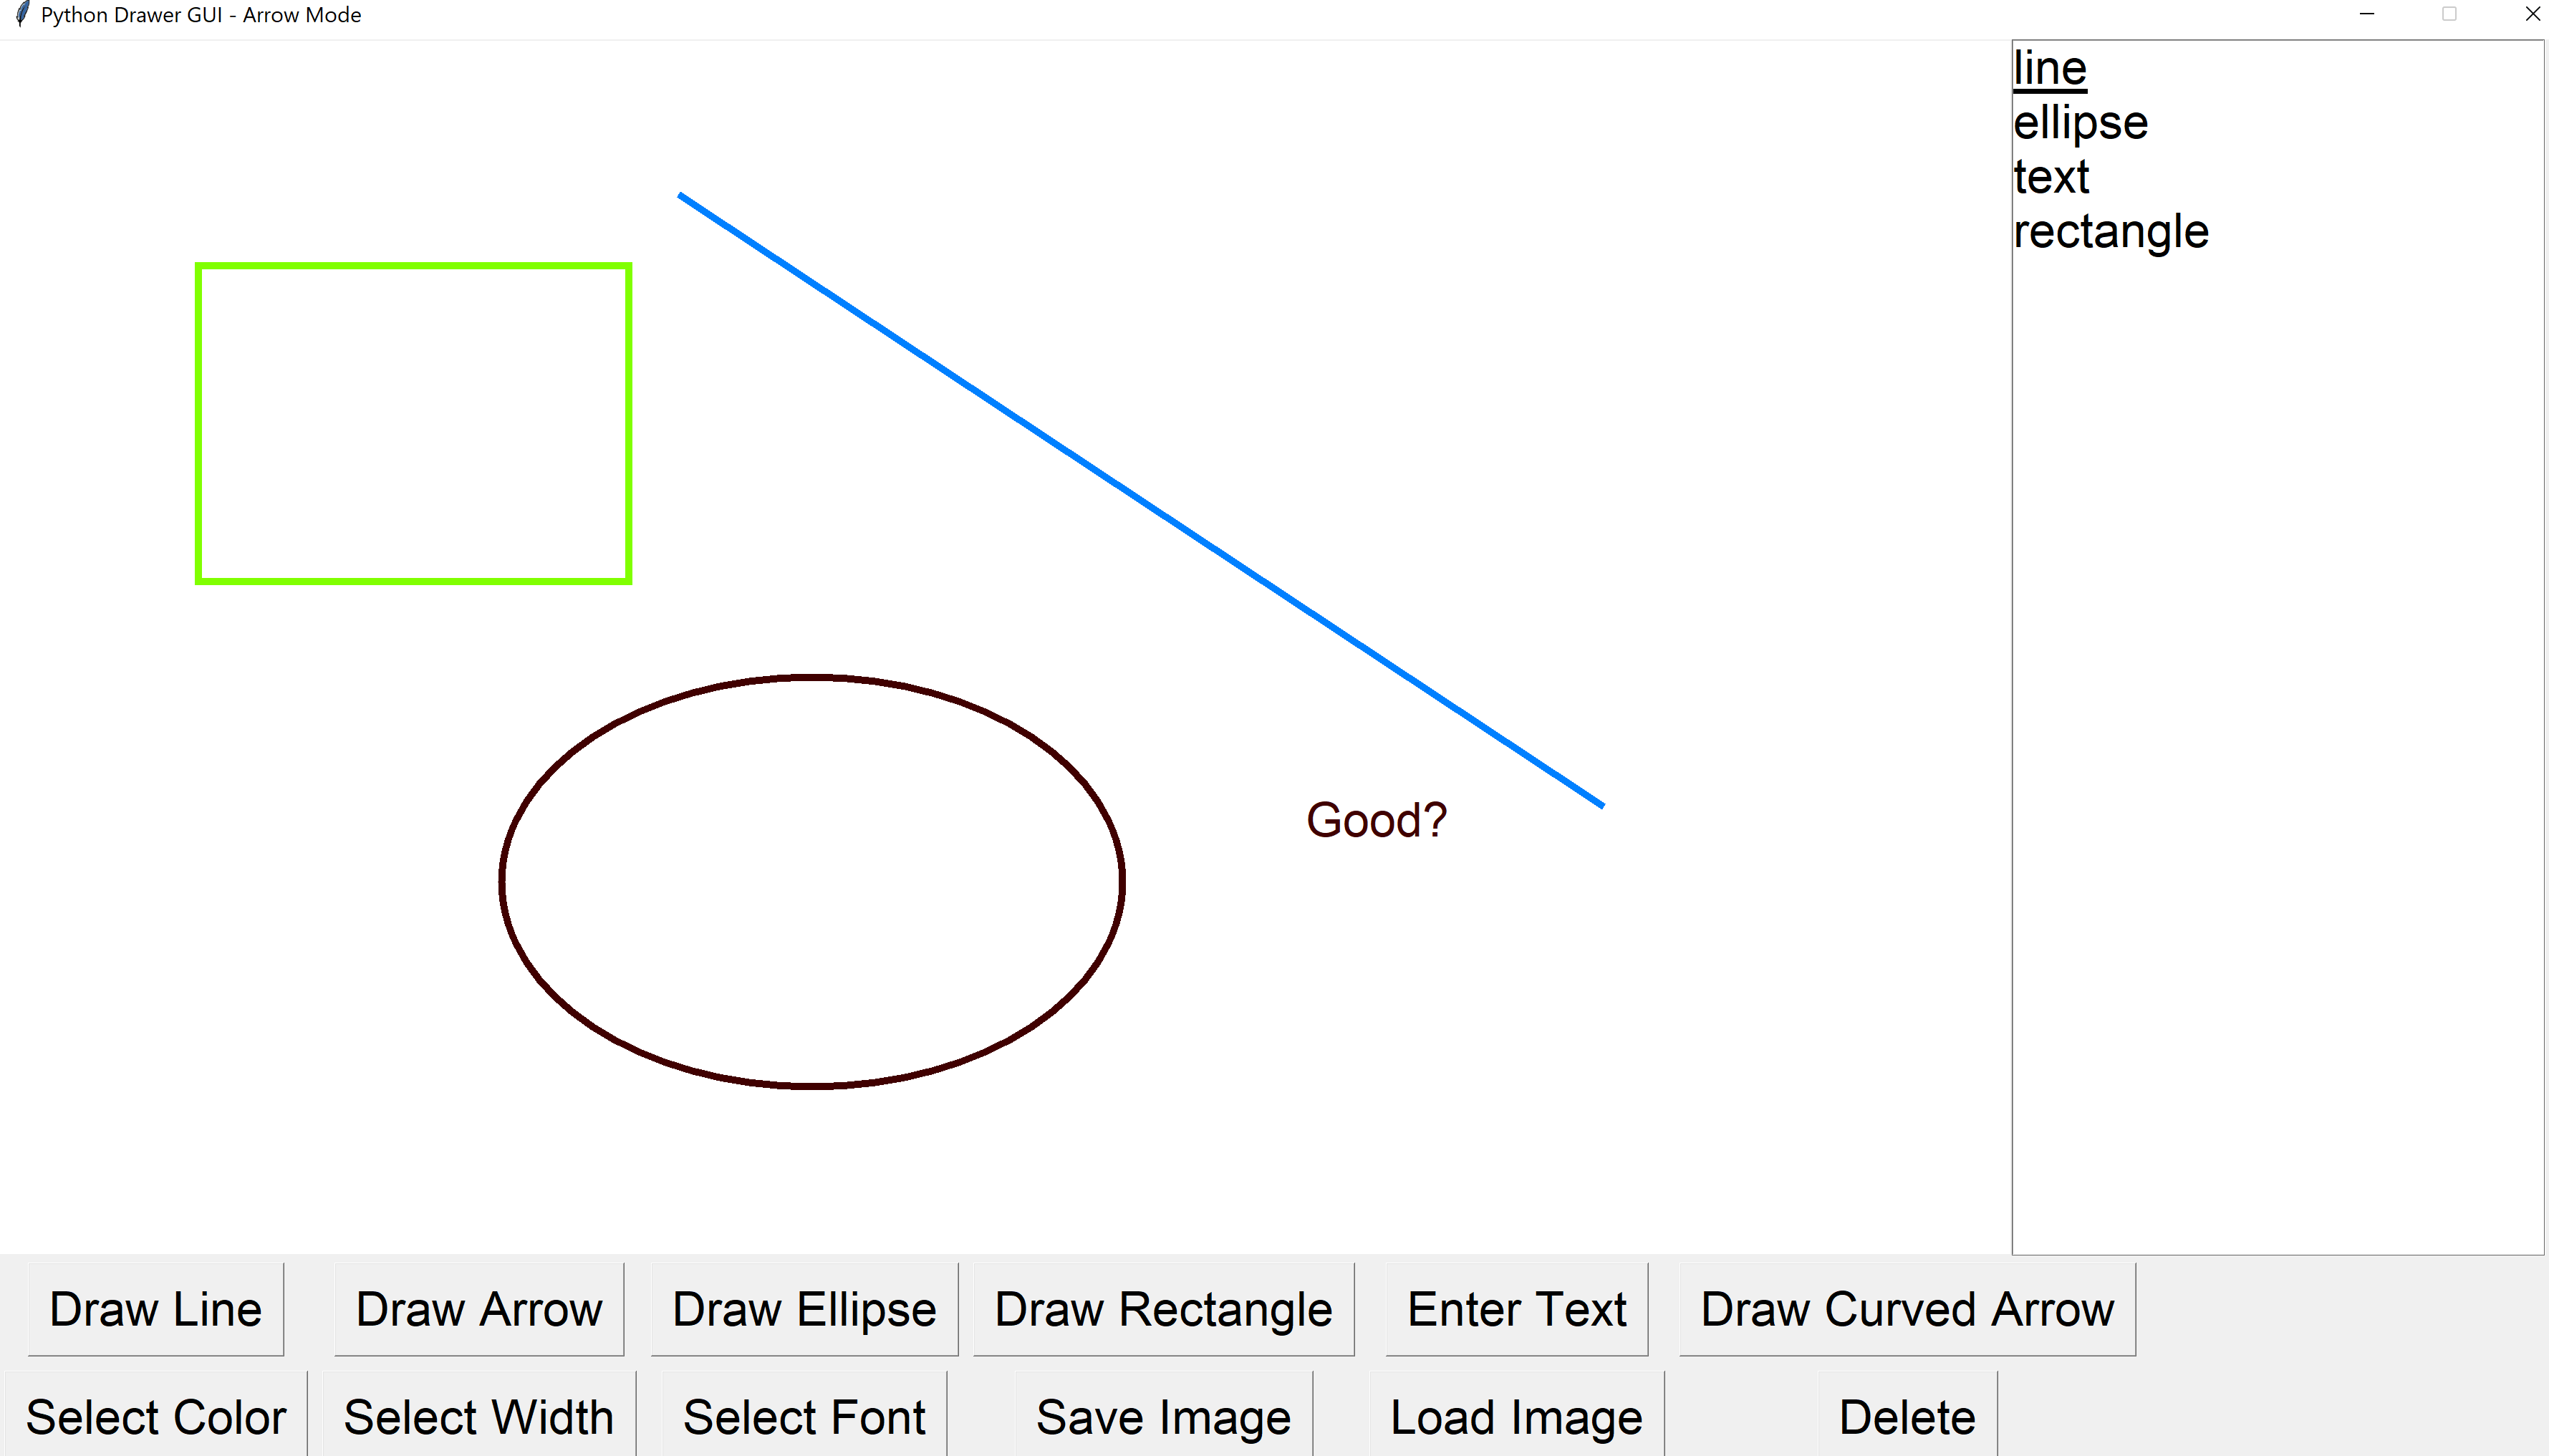
\includegraphics[width=0.45\linewidth]{figures/g5.png}
\end{AIbox}
\caption{The four pictures are (from top left to bottom right): Before selecting curved\_arrow, selecting curved\_arrow (in 5 seconds), 5 seconds after selecting curved\_arrow, after deleting curved\_arrow.}
\end{figure}


Although  \DV's code still needs some improvement for drawing curved arrows, it faithfully implements the natural language description in all aspects. \DV effectively uses color to emphasize the selected object, changing it to red for 5 seconds and then restoring it to the original color. \DV also maintains the consistency of the drawn objects, ensuring that they are removed from the drawing panel when they are deleted from the list. Moreover, \emph{\DV also remembers to show the intermediate object when a user drags the mouse to draw.}

\newpage
\subsection{Example for reverse engineering}
\label{appendix:reverse-engine}
\begin{tcolorbox}[colback=white!5!white,enhanced, breakable, colback=white!5!white]
\begin{minted}[breaklines, breaksymbol=, baselinestretch=1, fontsize=\tiny]{text}
Human: Now I have an executable file named easy_one in the home folder of my mac OS X laptop. Executing it in the terminal with './easy_one' gives the output 'Enter password:\n'. Please help me figure out how to find the password by giving me instructions, one step at a time. Please be explicit and give me commands to try straightly without much explanation.

AI: Yes, sir. The first command you should try is
file easy_one

Human: okay, it says
easy_one: Mach-O 64-bit executable x86_64
What's next?


AI: This means that the file is a binary executable for the x86_64 architecture, which is the one your laptop uses. The next command you should try is
strings easy_one

Human: This gives me
Enter the password...
Correct!
the password is: %s
wrong password

Anything interesting here?

......

AI: There are two possible ways to proceed from here. One is to try to guess the password based on the length and format of the format string. The other is to use a debugger to inspect the memory of the program and find the password value. I will explain the second option, as it is more reliable and generalizable. The next command you should try is
lldb ./easy_one

Human: (lldb) target create "./easy_one"
Current executable set to '/Users/yz/Downloads/easy_one' (x86_64).
(lldb) 

AI: This will launch the lldb debugger, which is a tool that allows you to control and examine the execution of a program. The next command you should try is
breakpoint set --name printf

Human: (lldb) breakpoint set --name printf
Breakpoint 1: where = libsystem_c.dylib`printf, address = 0x00007ff8002c70fc

AI: This will set a breakpoint at the printf function, which means that the program will stop whenever it calls this function. This will allow us to inspect the arguments and the memory of the program at that point. The next command you should try is
run

Human: (lldb) run
Process 33894 launched: '/Users/yz/Downloads/easy_one' (x86_64)
Process 33894 stopped
* thread #1, queue = 'com.apple.main-thread', stop reason = breakpoint 1.1
    frame #0: 0x00007ff81bb8e0fc libsystem_c.dylib`printf
libsystem_c.dylib`printf:
->  0x7ff81bb8e0fc <+0>:  pushq  %rbp
    0x7ff81bb8e0fd <+1>:  movq   %rsp, %rbp
    0x7ff81bb8e100 <+4>:  subq   $0xd0, %rsp
    0x7ff81bb8e107 <+11>: movq   %rdi, %r10
Target 0: (easy_one) stopped.

AI: This will run the program until it hits the breakpoint. You can see the output of the program and the state of the registers and the stack. The next command you should try is
register read rdi

Human: (lldb) register read rdi
        rdi = 0x0000000100000f66  "Enter the password...\n"

......

Human: Here is the assembly of the main function:
...

0000000100000e42         movsx      eax, byte [rbp+var_110]
0000000100000e49         movsx      ecx, byte [rbp+var_107]
0000000100000e50         cmp        eax, ecx
0000000100000e52         jne        loc_100000e82

0000000100000e58         lea        rsi, qword [rbp+var_110]
0000000100000e5f         lea        rdi, qword [aCorrectnthePas]                ; argument "format" for method imp___stubs__printf, "Correct!\\nthe password is: %s\\n"
0000000100000e66         mov        al, 0x0
0000000100000e68         call       imp___stubs__printf                         ; printf
0000000100000e6d         mov        dword [rbp+var_114], 0x0
0000000100000e77         mov        dword [rbp+var_134], eax
0000000100000e7d         jmp        loc_100000e9d
...

Have you found anything useful?

AI: Yes, sir. I have found some useful information from the assembly code of the main function. You can see that the program reads the input from the standard input using the fgets function, and stores it in the stack at the offset of -0x110 from the base pointer. Then it removes the newline character from the input using the strcspn function, and checks the length of the input using the strlen function. If the length is not equal to 10, it calls the _wrong_password function. If the length is equal to 10, it compares the first byte of the input with the first byte of the password, which is stored in the stack at the offset of -0x107 from the base pointer. If they are not equal, it calls the _wrong_password function. If they are equal, it prints the password using the printf function. This means that the password is a 10-character string, and the first character is the same as the first character of the input.

Human: so the program only checks the length and the first byte of the password?

AI: Yes, sir. That seems to be the case. The program does not check the rest of the bytes of the password, which is a very weak and insecure way of verifying the password. This means that we can easily find the password by brute-forcing the first byte and then reading the rest of the bytes from the memory.

Human: How to do that efficiently?

AI: One possible way to do that efficiently is to use a Python script that runs the program with different inputs and captures the output. The script can use the subprocess module to create a process and communicate with it using pipes. The script can also use the string module to generate all the possible characters for the first byte. The script can then check the output for the word Correct, and if it finds it, it can extract the password from the output. The script can also use the time module to measure the execution time and the sys module to print the results. Here is an example of such a script:

import subprocess
import string
......
# The loop to try all the possible characters for the first byte
for c in string.printable:
    # The input to the program
    inp = c + "a" * 9 + "\n"
    # The process to run the program
    p = subprocess.Popen(exe, stdin=subprocess.PIPE, stdout=subprocess.PIPE, stderr=subprocess.PIPE)
    # The output and the error of the program
    out, err = p.communicate(inp.encode())
    # The output as a string
    out = out.decode()
......

Human: great! Let me run your program. Here is the output: 
Password found: aaaaaaaaaa
Time elapsed: 0.15888214111328125 seconds

AI: Congratulations, sir. You have found the password using the Python script. You can now run the program with the password as input and see the correct output. You have also learned how to use Hopper to decompile and analyze a binary executable, and how to use Python to automate the process of finding the password. I hope you enjoyed this challenge and learned something new. Thank you for using my service. Have a nice day.
\end{minted}
\end{tcolorbox}
%\caption{}
%\label{fig:reverse-engine}

\newpage
\subsection{Testing {\DV}'s ability to execute (pseudo) code}
\label{sec:code_a5}
We ask {\DV} to execute the following pseudo code:
\begin{figure}[H]
\begin{AIbox}{\DV}
{\bf Prompt:} \begin{minted}[breaklines, breaksymbol=, baselinestretch=1, fontsize=\scriptsize]{python}
function f: input num1, num2, p.
assign val <- num1 * num2 + p
assign ret1 <- val % 10
assign ret2 <- val // 10
we return ret1, ret2 
end function.
function g: input: array1, array2.
m is the length of array1.
n is the length of array2.
p <- 0
r is a all zero array of length m + n+ 1
loop i from 0 to n - 1.
loop j from 0 to m - 1.
assign p <- r[i + j]
call f with input array1[i], array2[j] and p
we get ret1, ret2 as the return value.
update r[j + i] <- ret1
add r[j + i + 1] by ret2.
end loop
end loop
finally, we return r.
end g
What is the output of g on [...], [...]? Compute it with intermediate steps.
\end{minted}
\end{AIbox}
\caption{Measuring \DV's pseudo code execution ability.}
\label{fig:pseudocode2}
\end{figure}

 The $g$ takes two input arrays, the output is obtained by reversing and concatenating the digits of two arrays and then multiplying them. We fix one input array to a length $4$ array, with each element randomly sampled from $1-9$, and vary the length of the other array. We obtain the following accuracy versus length/steps (step here means how many time the array $r$ will be updated.)
 \begin{figure}[H]
\centering
 \begin{tabular}{c|ccccc}
\toprule
Length/Steps & 4/32 & 6/48 & 8/64 & 10/80 & 12/96 \\
\midrule
\midrule
Accuracy (100 samples) & 95\% & 88\% & 78\% & 62\% & 54\% \\
\bottomrule
\end{tabular}
\end{figure}
\vspace{-0.3cm}

We can see that even with $96$ steps (\emph{when the output of the model approaches its token limit of 8129}), the model still manages to keep track of the array $r$ up to $54 \%$ (here, the accuracy means that the percentage of the input instances where the output is an exact match). Obviously, this is not acceptable as a compiler (executor) yet, but already a significant step towards an AGI compiler capable of executing pseudo code. 
%\ronen{comment that this works only if it outputs the result of each step?}

Indeed,  \DV \ can also apply its skills to pseudo-code by generating equivalent code in a specific programming language. This task is not challenging for \DV , as it has already shown its remarkable coding abilities follow from natural language instructions. In this section, our main point is to demonstrate that \DV \ can not only write code, but also understand how programming works and execute it correctly.


